\documentclass{beamer}
\usetheme{Montpellier}
\usecolortheme{seahorse}

\usepackage{amsmath}
\usepackage{centernot}
\usepackage{bm}
\usepackage{pifont}
\usepackage{tikz}

\usepackage{fancybox}

\newcommand{\cmark}{\ding{51}}
\newcommand{\xmark}{\ding{55}}

\newcommand{\T}{^\text{T}}
\newcommand{\N}{\text{N}}
\newcommand{\twolinecell}[2][c]{%
  \begin{tabular}[#1]{@{}c@{}}#2\end{tabular}}
\graphicspath{{images/}}

\newcommand{\redstar}{\textcolor{red}{*}}

\setlength{\tabcolsep}{0pt}

\setbeamercovered{invisible}

\newsavebox{\fmbox}
\newenvironment{fmpage}[1]
{\begin{lrbox}{\fmbox}\begin{minipage}{#1}}
{\end{minipage}\end{lrbox}\fbox{\usebox{\fmbox}}}

\AtBeginSection[]{
  \begin{frame}
  \vfill
  \centering
  \begin{beamercolorbox}[sep=8pt,center,shadow=true,rounded=true]{title}
    \usebeamerfont{title}\insertsectionhead\par%
  \end{beamercolorbox}
  \vfill
  \end{frame}
}


\graphicspath{{supporting_files/figs/}}

\title{Two Reasons to Model Phenotype\\ Mean and Variance in QTL Mapping}
\author{Robert Corty}
\institute{UNC Chapel Hill}
\date{BCB Colloquium\\\today}

\begin{document}

\begin{frame}
\titlepage
\end{frame}

\begin{frame}{Overview}
\tableofcontents
\end{frame}


\section*{Acknowledgements}
\begin{frame}\frametitle{Acknowledgements}
    \begin{minipage}{0.45\textwidth}
        {\small
        \textbf{Software:} CRAN package vqtl\\
        \textbf{Slides:} github.com/rcorty/BCB\_colloquium\\\\
        \textbf{Collaborators:}\\
        Lisa Tarantino\\
        Ethan Lange\\
        Leslie Lange\\
        Laura Raffield}
    \end{minipage}\hfill
    \begin{minipage}{0.45\textwidth}
        {\small
        \textbf{Valdar lab:}\\
        Will Valdar\\
        Greg Keele\\
        Dan Oreper\\
        Paul Maurizio\\
        Wes Crouse\\
        Yanwei Cai}
    \end{minipage}
\end{frame}


\section{Background}

\begin{frame}\frametitle{F2 Intercross Mapping Population}
    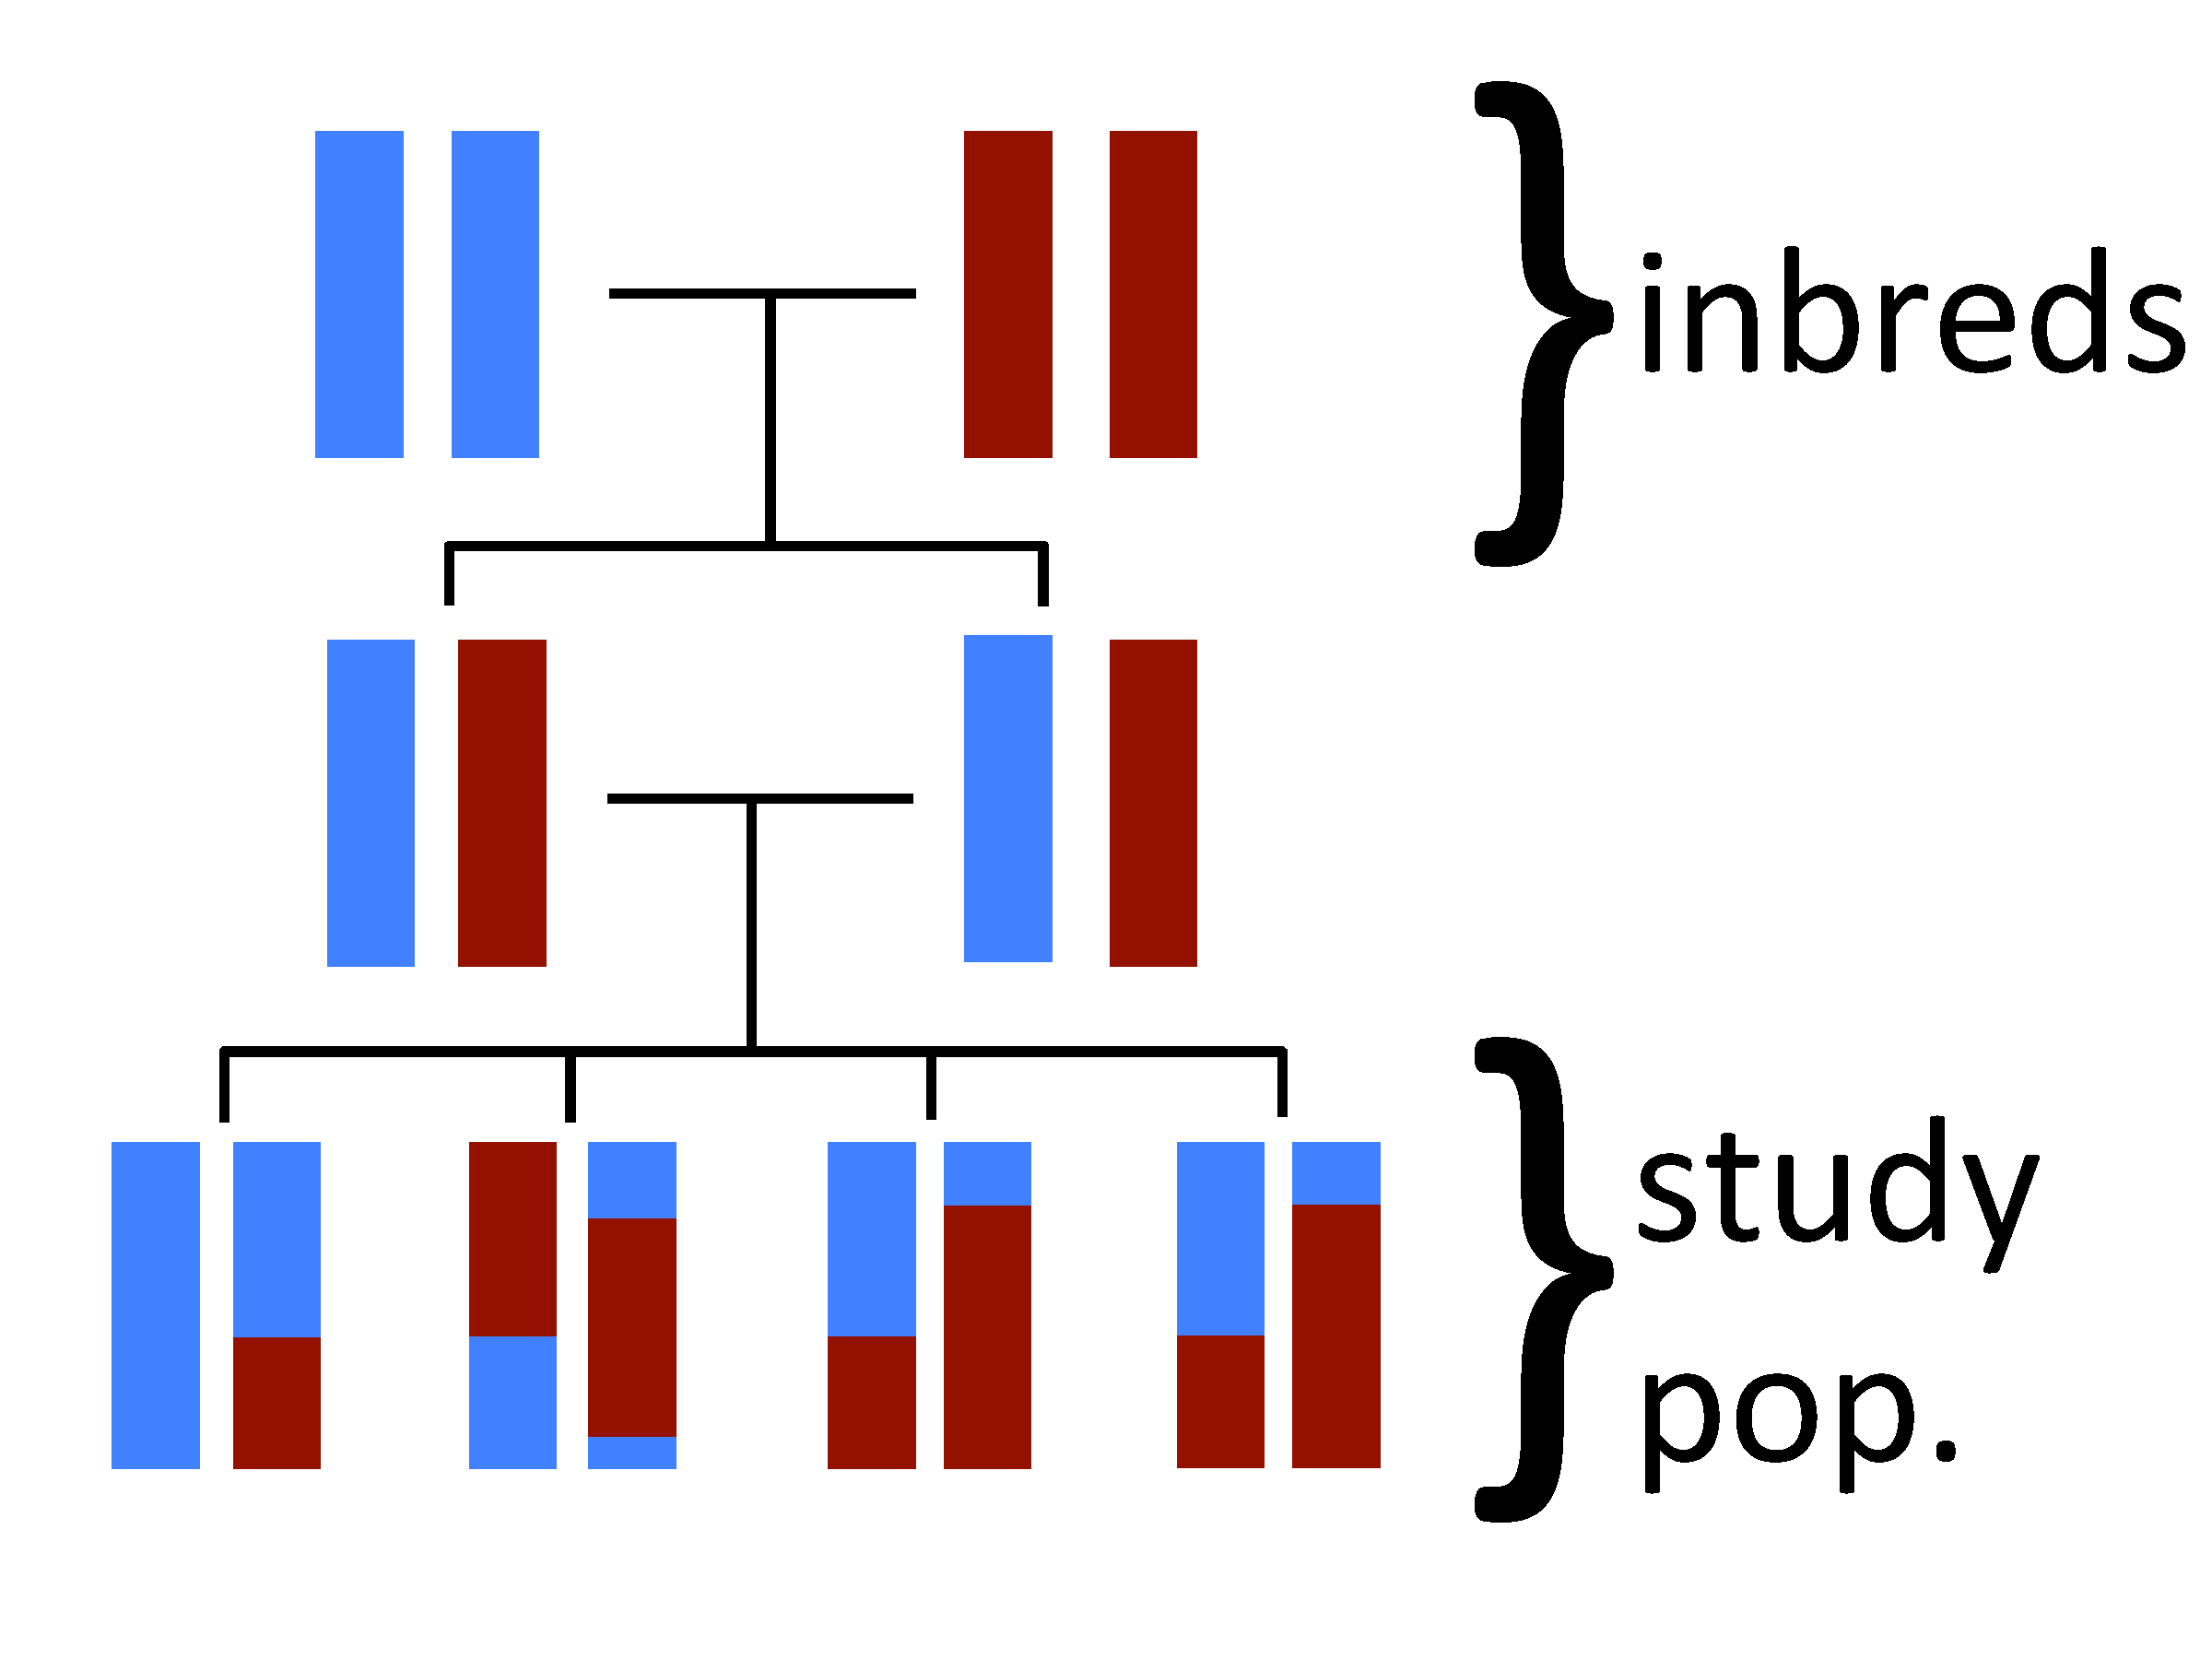
\includegraphics[width = 3in]{F2_diagram}
\end{frame}

\begin{frame}\frametitle{Current Approach to QTL Mapping}
    \begin{minipage}{0.3\textwidth}
        \begin{tikzpicture}
            \node[inner sep=0pt] (main_image) at (0,0) {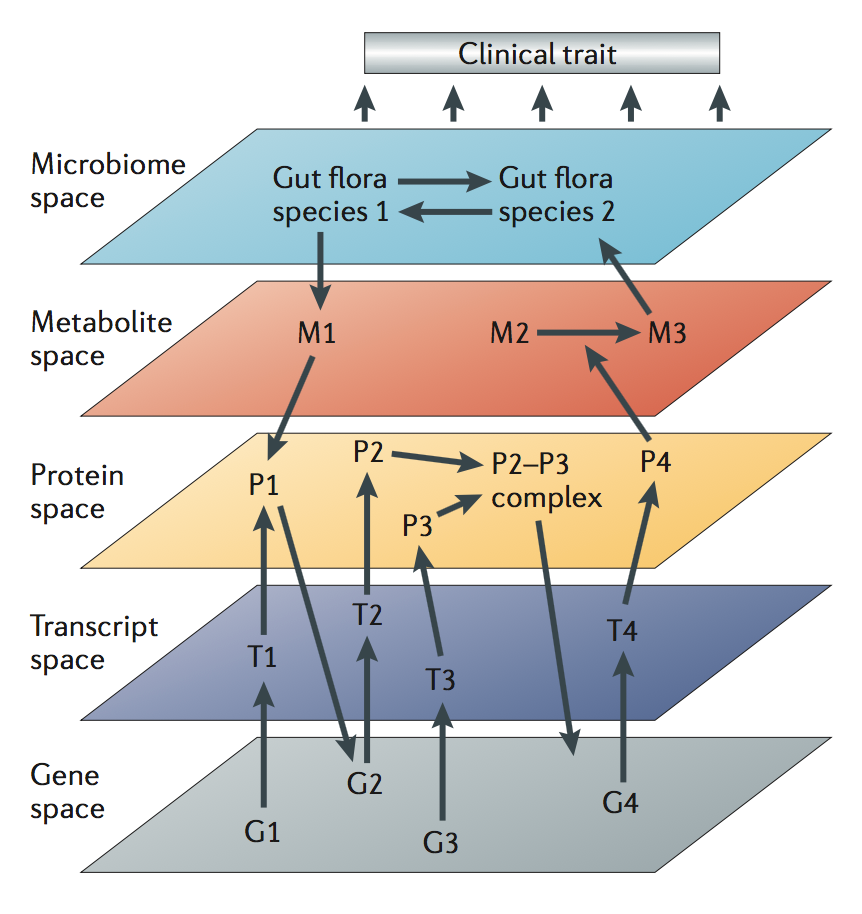
\includegraphics[width=2in]{systems_genetics}};
            \uncover<2>{\draw[red, ultra thick] (-2.5, -1.6) rectangle (-1.8, -2.4);}
            \uncover<2>{\draw[red, ultra thick] (-0.7, 2.2) rectangle (2.1, 2.6);}
            \uncover<2>{\draw[-latex, ultra thick, red] (-1.8, -2) to[out=0, in=-90] (0.8, 2.2);}
        \end{tikzpicture}
        {\scriptsize Civelek, 2014}
    \end{minipage}\hfill
    \begin{minipage}{0.4\textwidth}
        Truth:
        \begin{align*}
            y_i &= f(g_i, t_i, e_i, ...)
        \end{align*}
        \uncover<2>{Statistical Model:}
        \uncover<2>{
        \begin{align*}
            y_i &= m_i + \epsilon_i\\%&\sim \text{N}(m_i, \sigma^2)\\
            \epsilon_i &\sim \text{N}(0, \sigma^2)\\
            &\text{with}\\
            m_i &= \bm{x}_i\T\bm{\beta} + \bm{q}_i\T\bm{\alpha}

        \end{align*}
        }
    \end{minipage}
\end{frame}


\begin{frame}\frametitle{DGLM Model}
    \begin{minipage}{0.4\textwidth}
        Constant variance\\QTL Mapping Model:
        \begin{align*}
            y_i &= m_i + \epsilon_i\\
            \epsilon_i &\sim \text{N}(0, \sigma^2)\\
            &\text{with}\\
            m_i &= \bm{x}_i\T\bm{\beta} + \bm{q}_i\T\bm{\alpha}
\\
        \end{align*}
        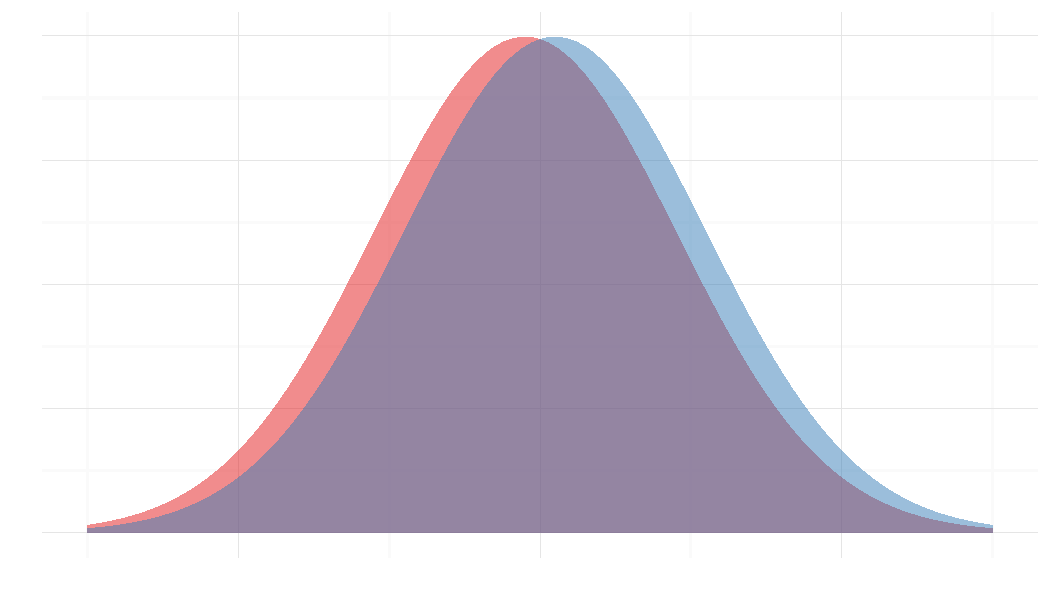
\includegraphics[width = 2in]{mean_effect_two_groups}
    \end{minipage}\hfill
    \pause
    \begin{minipage}{0.4\textwidth}
        Heterogeneous variance\\ QTL Mapping Model:
        \begin{align*}
            y_i &= m_i + \epsilon_i\\%&\sim \N(m_i, \exp(v_i)^2)\\
            \epsilon_i &\sim \text{N}(0, \text{exp}(v_i)^2)\\
            &\text{with}\\
            m_i &= \bm{x}_i\T\bm{\beta} + \bm{q}_i\T\bm{\alpha}\\
v_i &= \bm{z}_i\T\bm{\gamma} + \bm{q}_i\T\bm{\theta}

        \end{align*}
        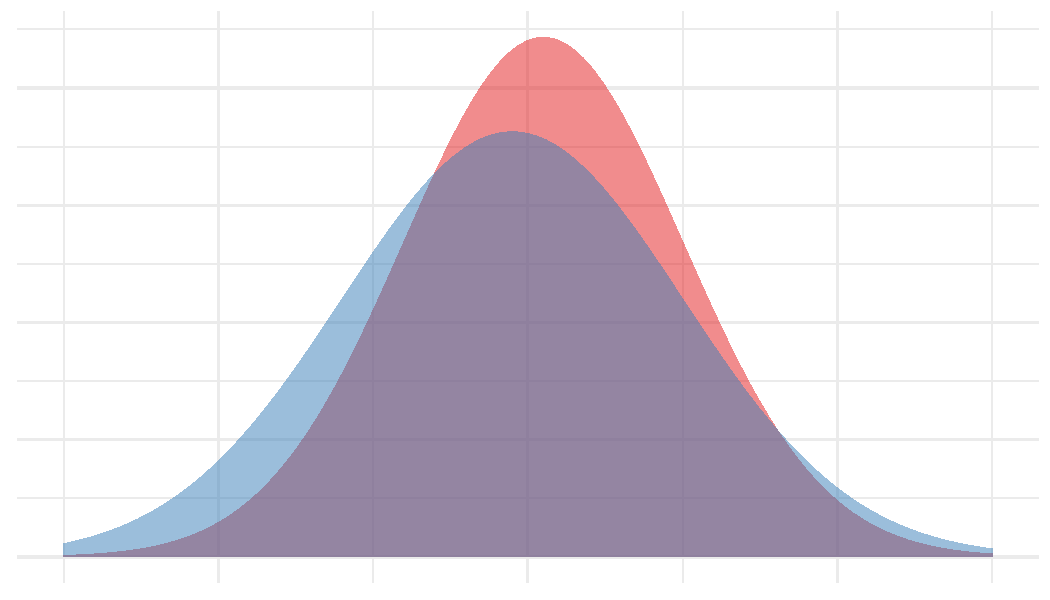
\includegraphics[width = 2in]{meanvar_effect_two_groups}
    \end{minipage}
\end{frame}


\begin{frame}\frametitle{Credits}
    \begin{center}
        \shadowbox{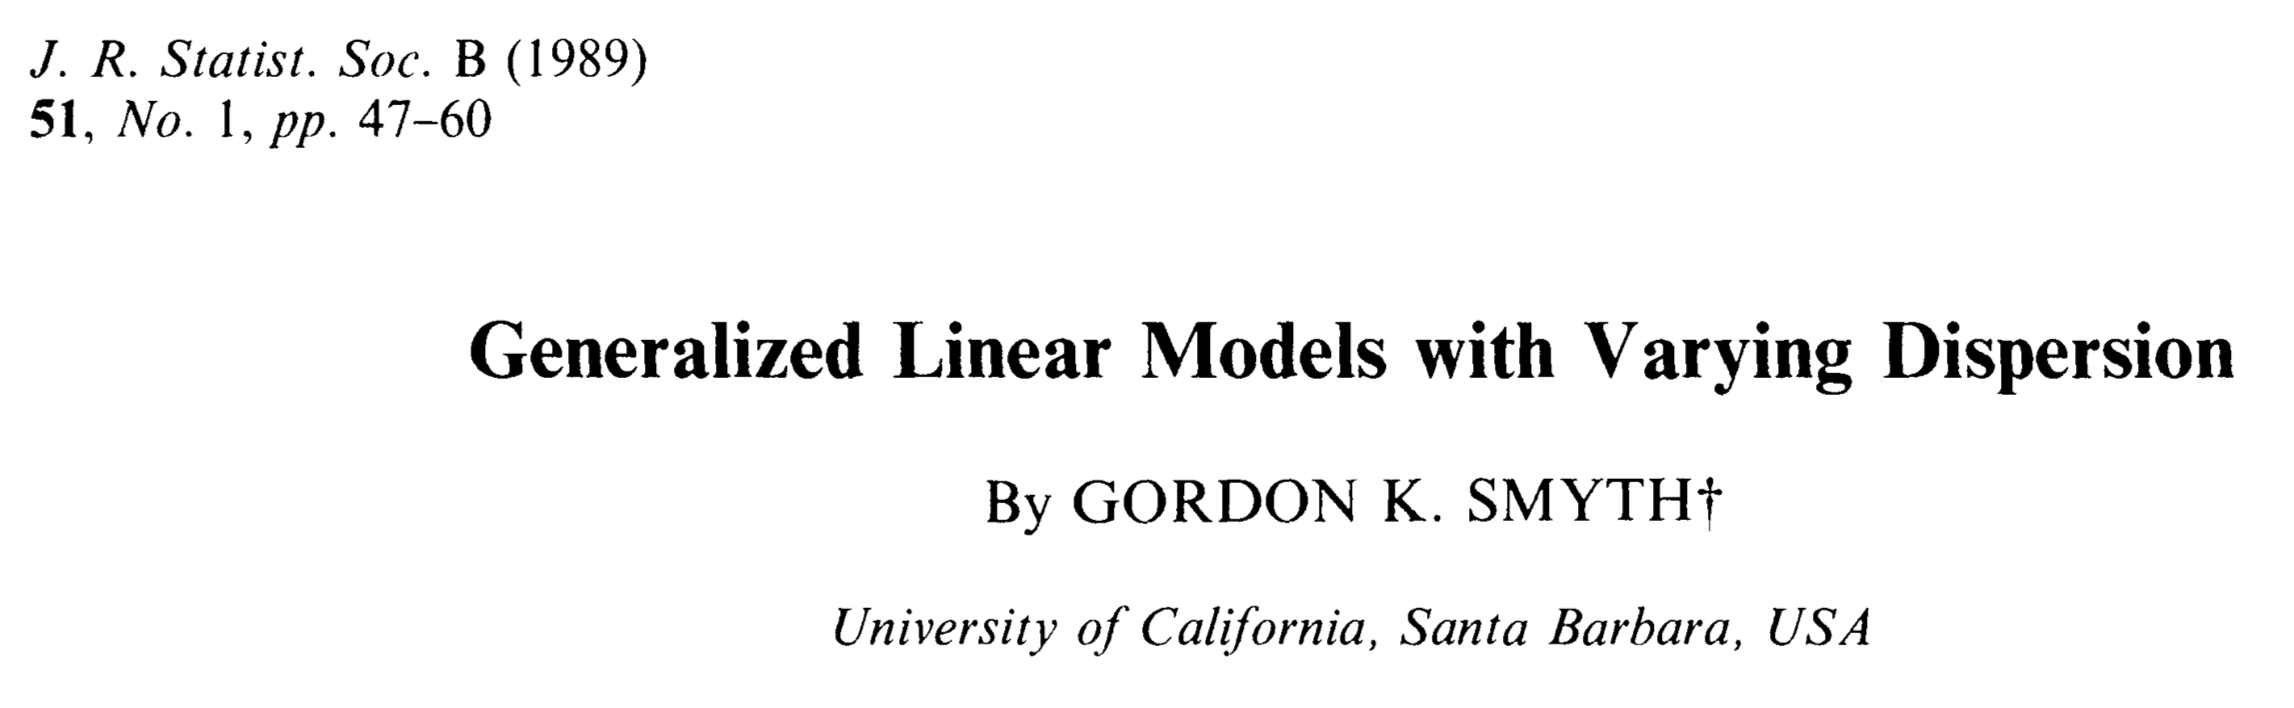
\includegraphics[width=0.7\textwidth]{Smyth1989}}\\\vspace{1em}
        \shadowbox{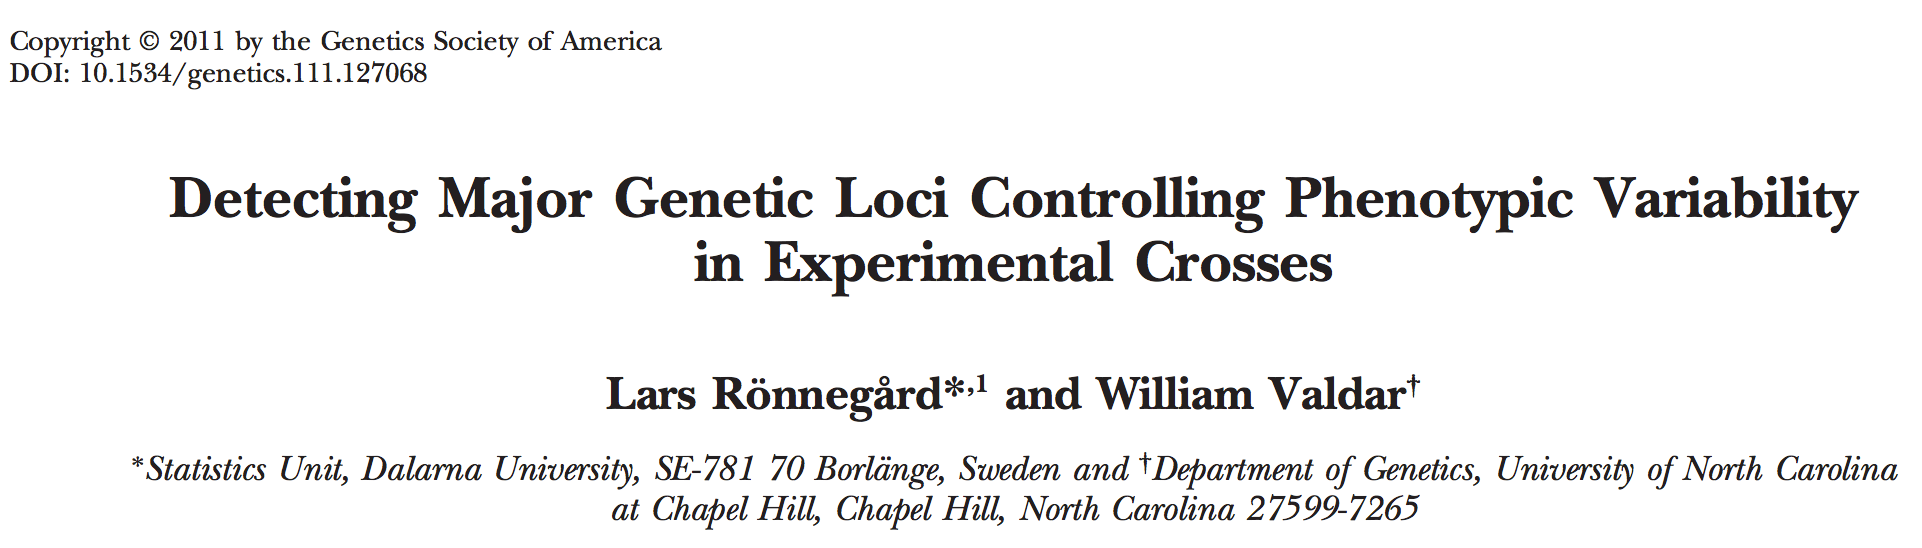
\includegraphics[width=0.7\textwidth]{RonnegardValdar}}
    \end{center}
\end{frame}


% \begin{frame}\frametitle{Two Patterns}
%     \begin{minipage}{0.4\textwidth}
%         \begin{center}
%             mean heterogeneity\\
%             \vspace{1cm}
%             \includegraphics<1>[width = 2in]{gray_mean_effect_two_groups}
%             \includegraphics<2>[width = 2in]{mean_effect_two_groups}
%             \includegraphics<3>[width = 2in]{gray_mean_effect_seven_groups}
%             \includegraphics<4-7>[width = 2in]{mean_effect_seven_groups}
%         \end{center}
%     \end{minipage}\hfill
%     \begin{minipage}{0.4\textwidth}
%         \begin{center}
%             variance heterogeneity\\
%             \vspace{1cm}
%             \includegraphics<1-4>[width = 2in]{gray_var_effect_two_groups}
%             \includegraphics<5>[width = 2in]{var_effect_two_groups}
%             \includegraphics<6>[width = 2in]{gray_var_effect_seven_groups}
%             \includegraphics<7>[width = 2in]{var_effect_seven_groups}
%         \end{center}
%     \end{minipage}
% \end{frame}

% 
% \begin{frame}\frametitle{Two Patterns}
%     \begin{minipage}{0.4\textwidth}
%         \hspace{2.2cm}mQTL\\\\
%         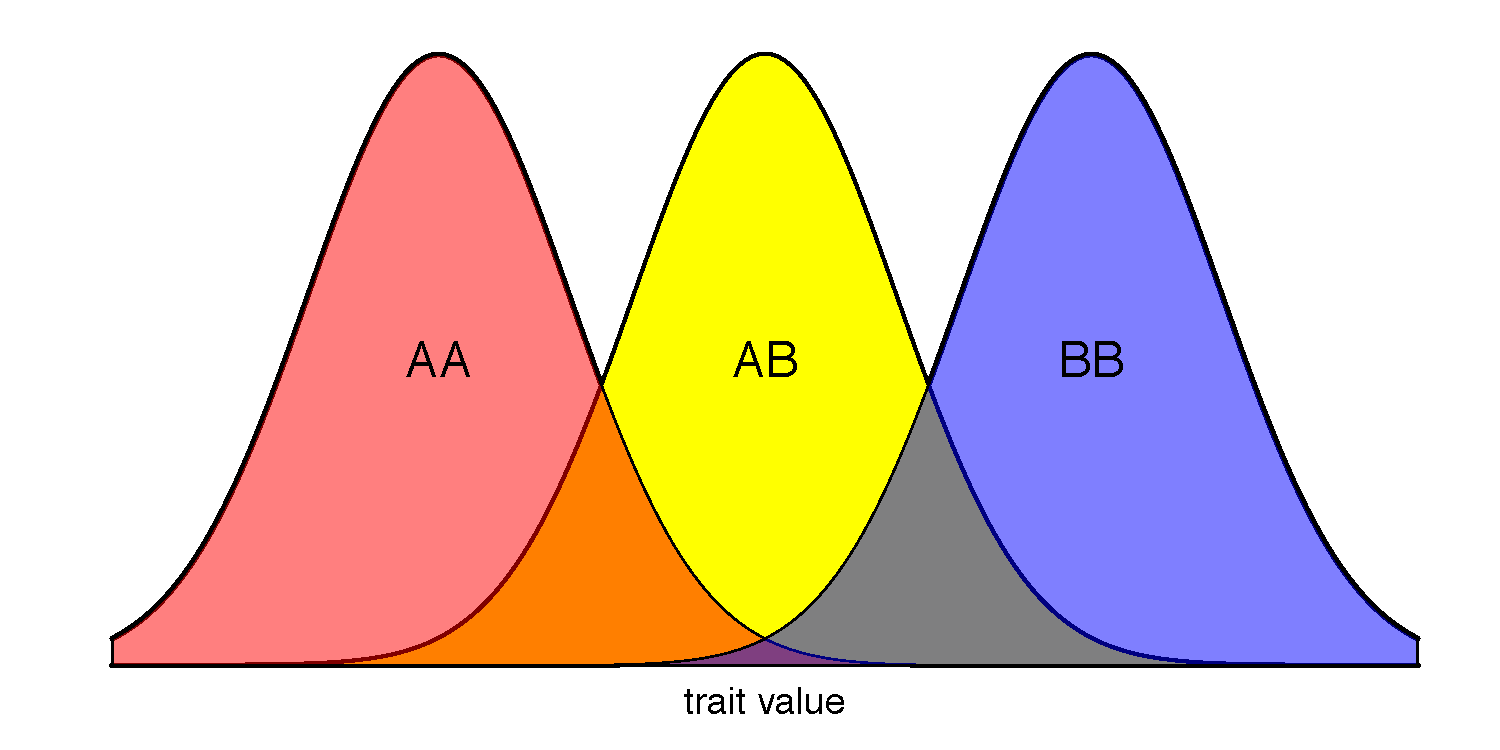
\includegraphics[width = 2in]{mQTL}
%     \end{minipage}\hfill
%     \begin{minipage}{0.4\textwidth}
%         \hspace{2.2cm}vQTL\\\\
%         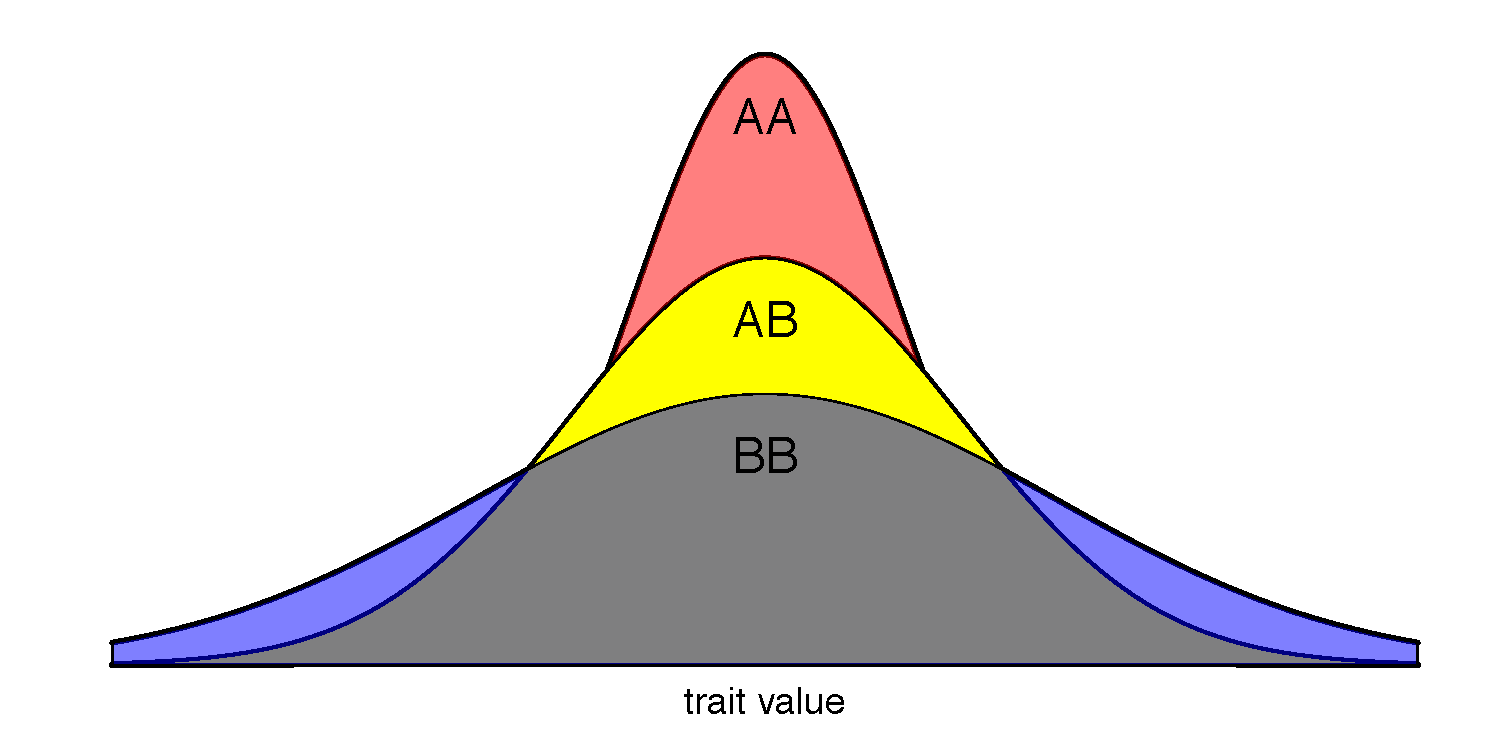
\includegraphics[width = 2in]{vQTL}
%     \end{minipage}
% \end{frame}




\section{Mean QTL Mapping}


\begin{frame}\frametitle{Nuisance Variance Heterogeneity}
    
    Could some levels of nuisance covariates yield more precise observations than others?
    
    \begin{itemize}
        \item Technician
        \item Day
        \item Apparatus
        \item Sex of model organism
    \end{itemize}
    
    Up-weight those observations.\\
    Down-weight the (otherwise) high leverage points.
    
\end{frame}


\begin{frame}\frametitle{Significance vs. Zero-ness}

    $p > 0.05 \centernot\implies \beta = 0$\\
    
    \vspace{1em}
    If we wouldn't trust a result that requires excluding some covariate, we should probably model it.
\end{frame}


\begin{frame}\frametitle{Example 1}
    \includegraphics<1>[width = \textwidth]{aric_BMI_gray.pdf}
    \includegraphics<2>[width = \textwidth]{aric_BMI_by_sex.pdf}\\
    Implications for study design
\end{frame}


\begin{frame}\frametitle{Example 2}
    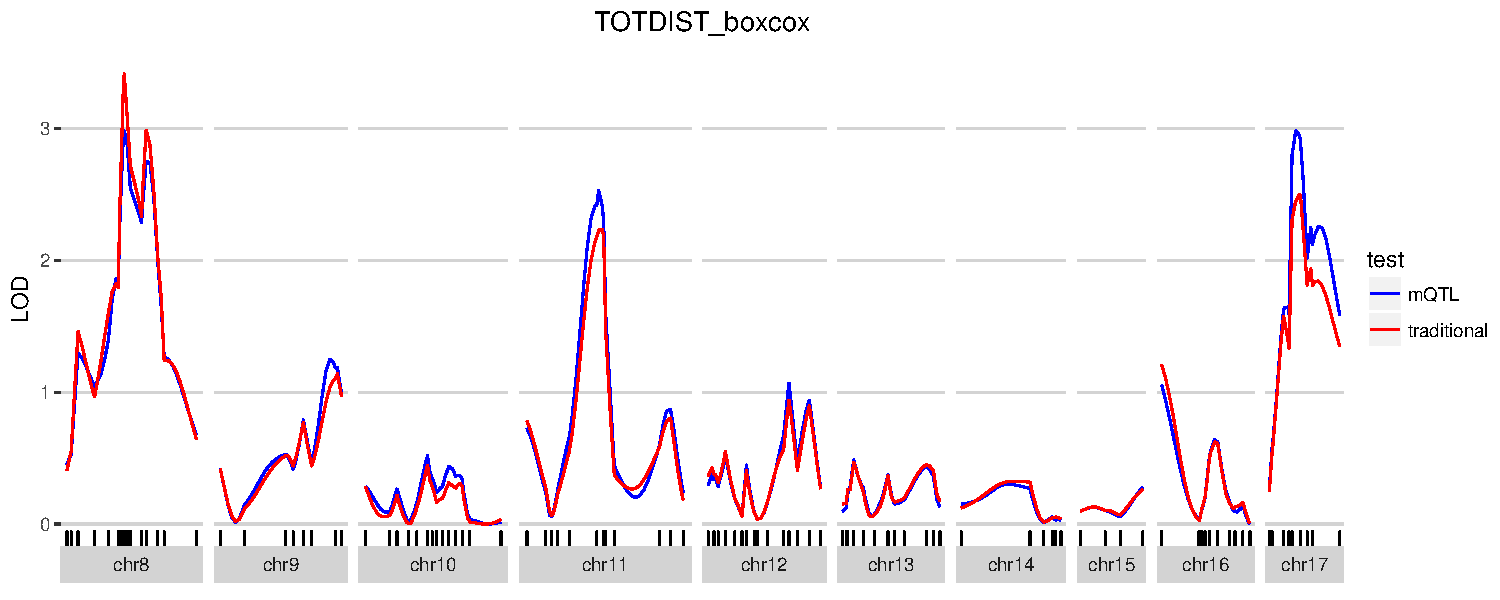
\includegraphics[width=\textwidth]{TOTDIST_boxcox}
\end{frame}


\begin{frame}\frametitle{Implications for Power}

    \begin{minipage}{0.45\textwidth}
        \begin{center}
            Homogenous variance\\scenario:
            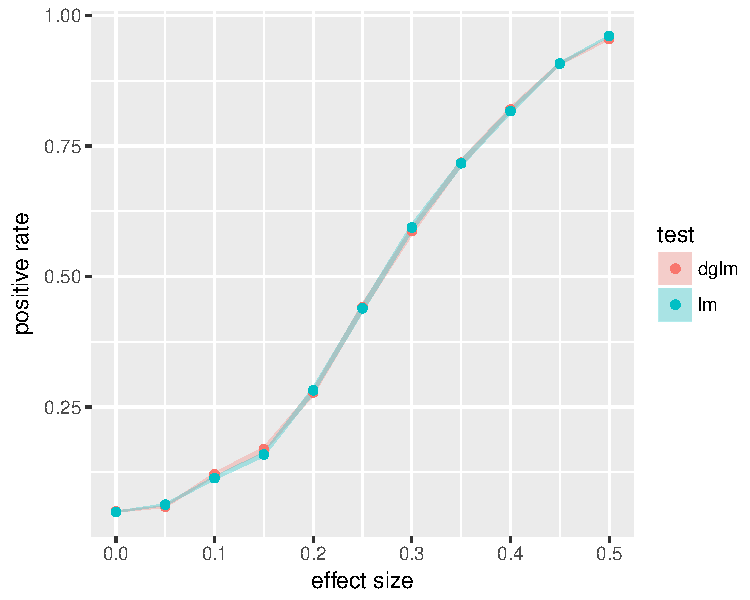
\includegraphics[width = \textwidth]{hom_power}
        \end{center}
    \end{minipage}\hfill
    \begin{minipage}{0.45\textwidth}
        \begin{center}
            Heterogeneous variance\\scenario:
            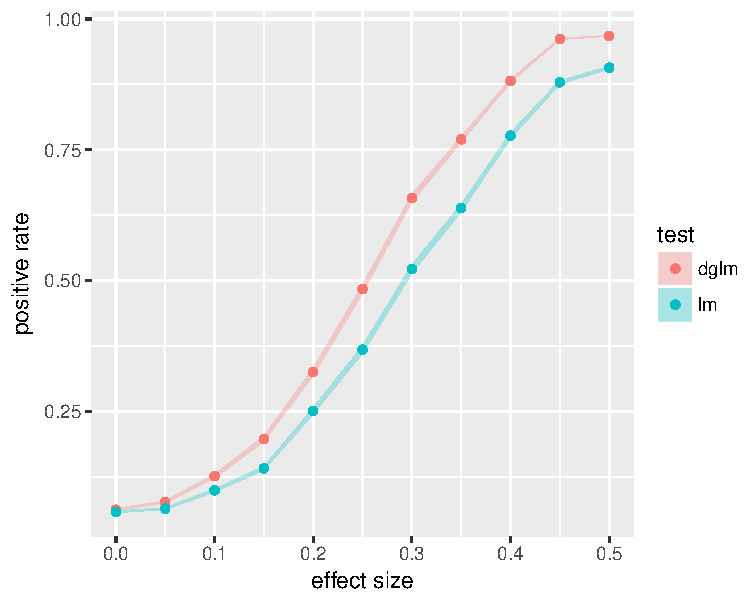
\includegraphics[width = \textwidth]{het_power}
        \end{center}
    \end{minipage}
    

\end{frame}



\section{Variance QTL Mapping}

% gxE unknown E
\begin{frame}\frametitle{GxE}
    \begin{center}
        \includegraphics<1>[width = 0.5\textwidth]{vQTL_unexplained}
        \includegraphics<2>[width = 0.5\textwidth]{vQTL_explained}
    \end{center}
\end{frame}

% liability threshold or uniformity
\begin{frame}\frametitle{Liability-Threshold Model}

    \begin{minipage}{0.45\textwidth}
        \begin{center}
            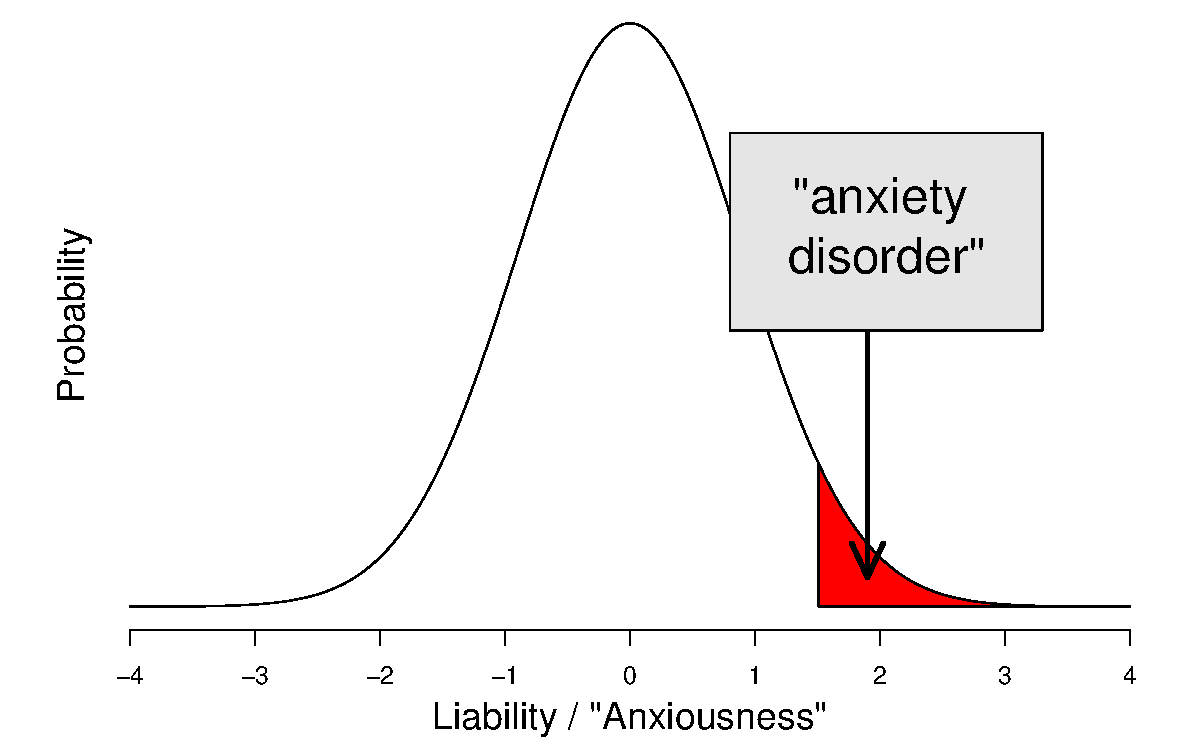
\includegraphics[width = \textwidth]{liability_threshold_low}
        \end{center}
    \end{minipage}\hfill
    \begin{minipage}{0.45\textwidth}
        \begin{center}
            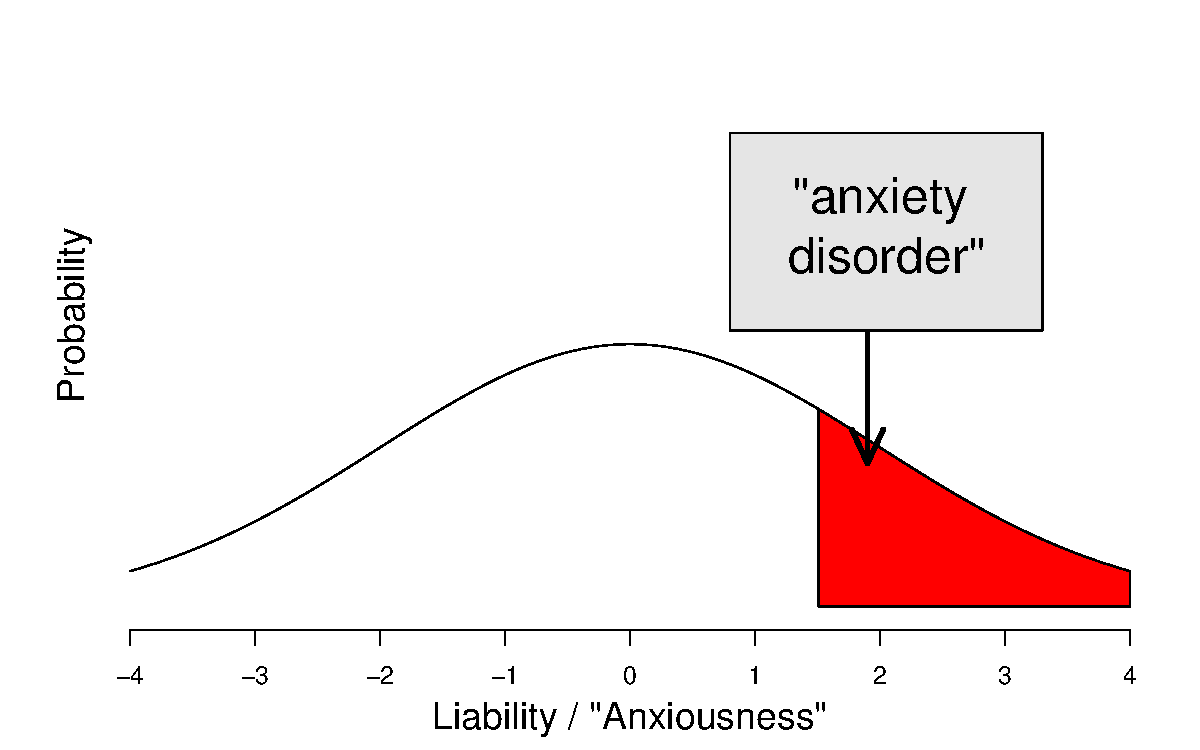
\includegraphics[width = \textwidth]{liability_threshold_high}
        \end{center}
    \end{minipage}
    
\end{frame}

% finding

\begin{frame}\frametitle{Example 1}

    \begin{center}
        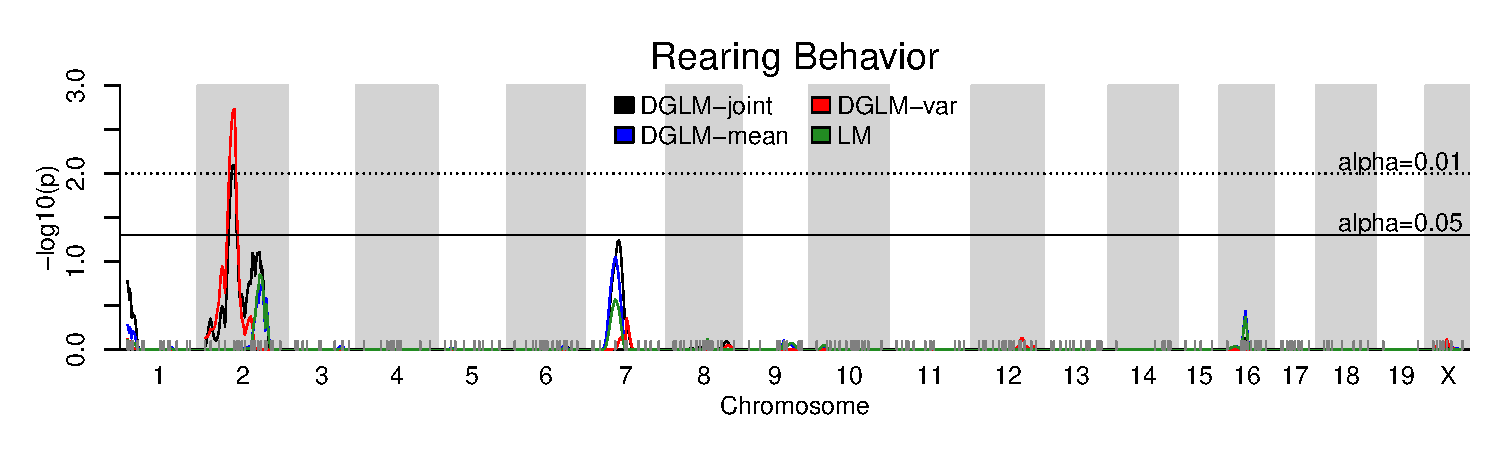
\includegraphics[width = \textwidth]{manufig_rearing}
    \end{center}
    
\end{frame}


\section{Unsolicited Advice}

\begin{frame}\frametitle{Unsolicited Advice}

    \begin{minipage}{0.45\textwidth}
        \begin{center}
            
\includegraphics[width = 0.8\textwidth]{falconer}
        \end{center}
    \end{minipage}\hfill
    \begin{minipage}{0.5\textwidth}
        \begin{itemize}
            \item Work for someone you like.
            \item Do an easy project first.
            \item Read Falconer.
        \end{itemize}
        \vspace{1em}
        Gratten 2016, Nature Genetics\\
        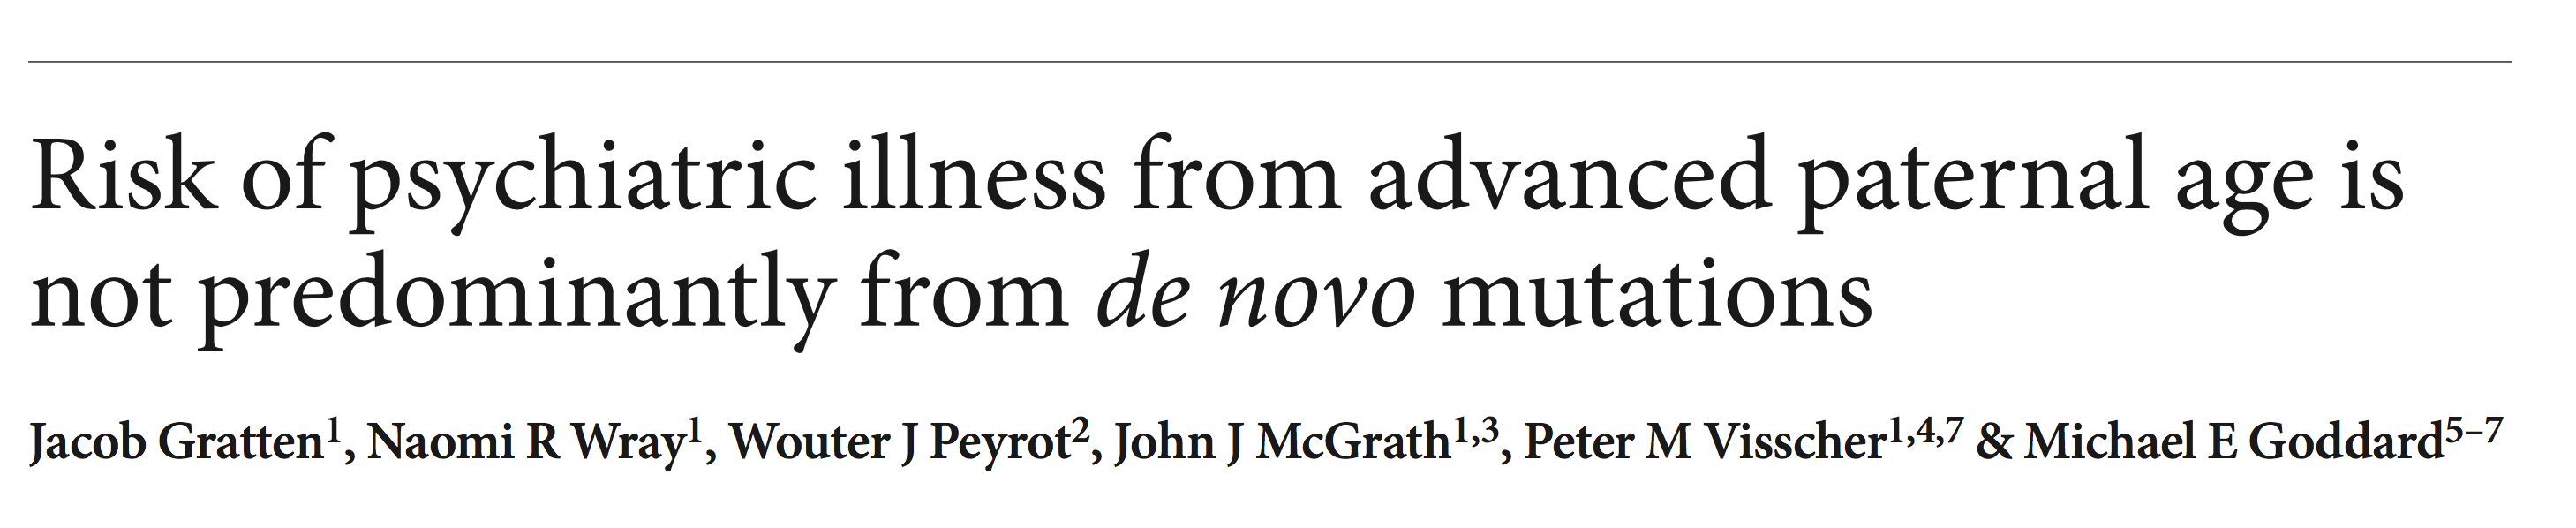
\includegraphics[width = 0.8\textwidth]{wray}
    \end{minipage}
    
\end{frame}



% 
% \begin{frame}\frametitle{LM and DGLM, Conceptually}
%   \begin{columns}[c]
%     \begin{column}{.5\textwidth}
%       \begin{center}
%         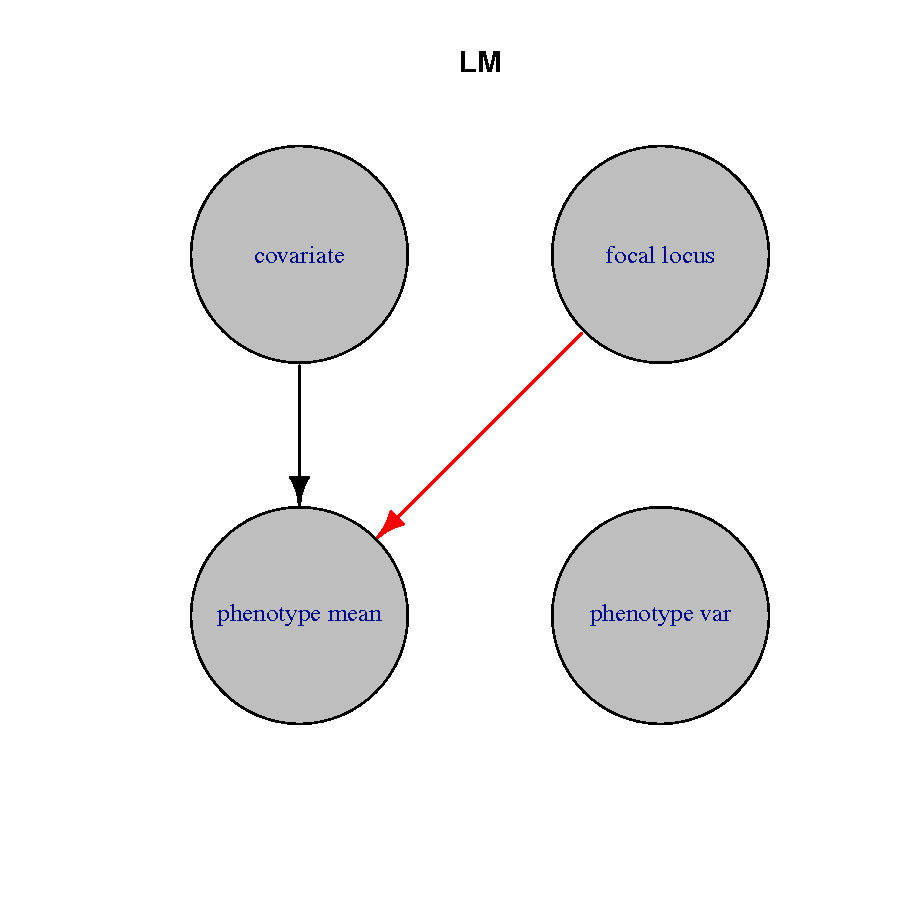
\includegraphics[width = 0.6\textwidth]{lm}\\
%         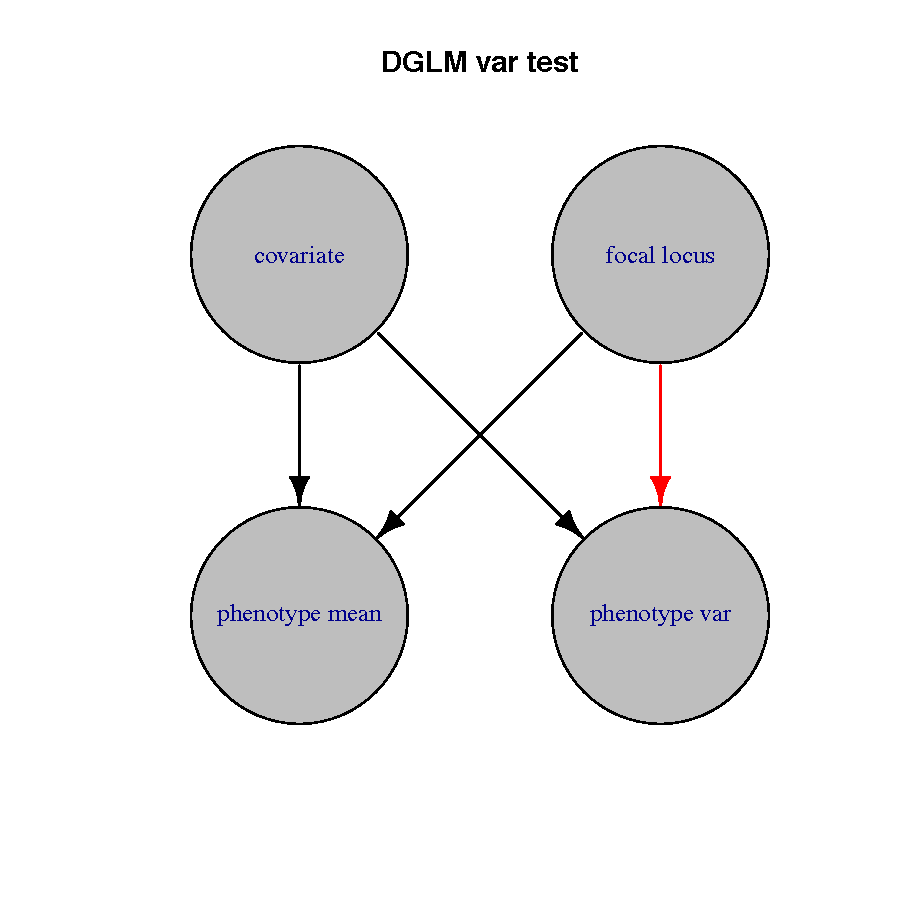
\includegraphics[width = 0.6\textwidth]{dglm_v}
%       \end{center}
%     \end{column}
%     \begin{column}{.5\textwidth}
%       \begin{center}
%         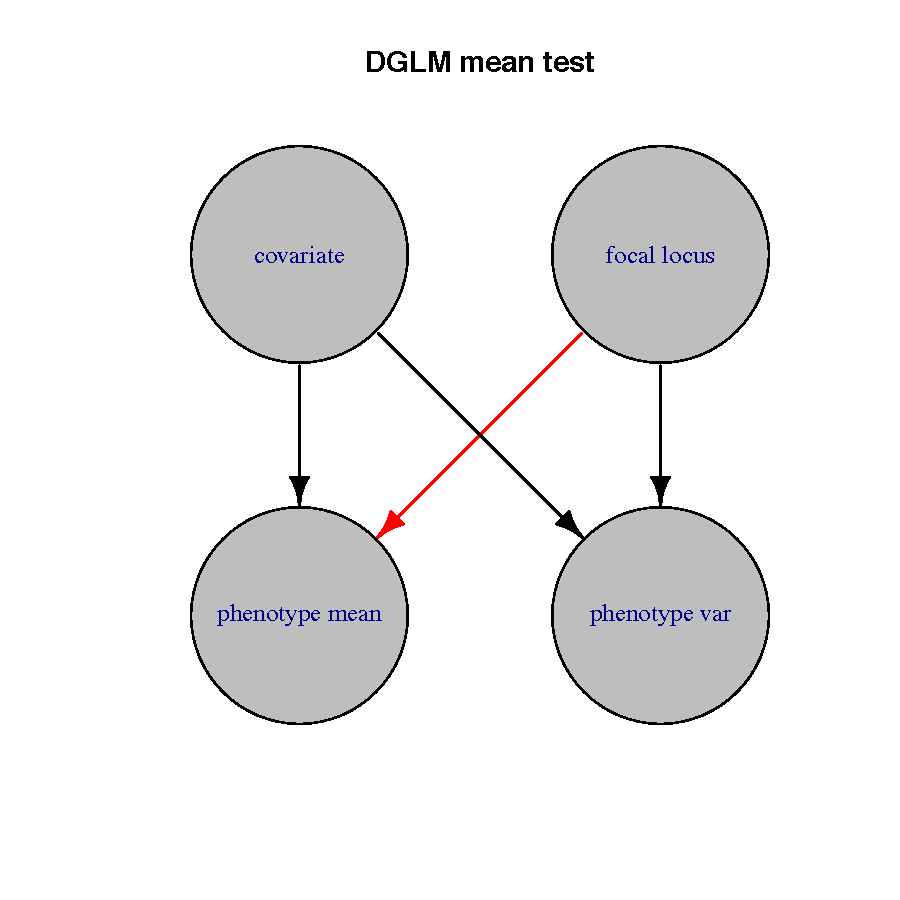
\includegraphics[width = 0.6\textwidth]{dglm_m}\\
%         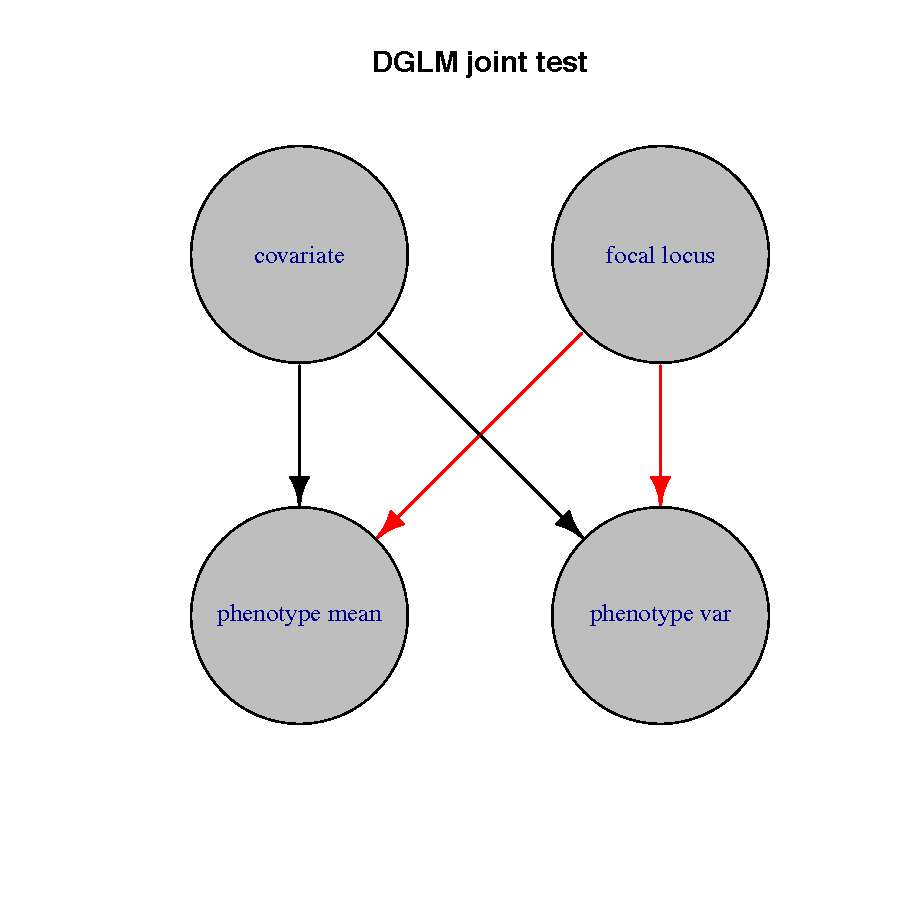
\includegraphics[width = 0.6\textwidth]{dglm_j}
%       \end{center}
%     \end{column}
%   \end{columns}
% \end{frame}
% 
% 
% 
% \begin{frame}\frametitle{Novelty}
%   \begin{enumerate}
%     \item Model additive and dominance genetic effects, test them alone or jointly
%     \item Test for mean and variance effects jointly
%     \item Multiple testing correction via FWER
%     \item Plotting in terms of -logP for standardizing evidence across tests
%     \item Modeling covariate effects in the null and alternative (e.g. testing mean -- model sex effect and locus effect on trait variance in mean and alt)
%   \end{enumerate}
% \end{frame}
% 
% 
% \begin{frame}\frametitle{Multiple Testing Correction}
%   \begin{enumerate}
%     \item How Many Tests?
%       \begin{itemize}
%         \item 1069 measured or inferred markers (but they are correlated)
%         \item 20 chromosomes (but there is variation within chromosomes)
%       \end{itemize}
%     \item FWER
%       \begin{itemize}
%         \item one genome scan is a family
%         \item compute LRS from null model vs. alternative model
%         \item compare to maximum LRS per genome from null model vs. randomized alternative model
%         \item conditional randomization scheme:  permute only the treatment allocation for the effect being tested
%         \item this scheme creates a null dataset that maintains as much of the character of the original phenotype as possible
%       \end{itemize}
%   \end{enumerate}
% \end{frame}
% 
% 
% 
% 
% \begin{frame}\frametitle{Results (1)}
%   \begin{itemize}
%     \item[1)] Reproduce published analysis of Bailey2008\\
%     \begin{itemize}
%       \item[-] Reproduced LOD scores but not threshold of 3.3.
%       \item[-] Reproducible research
%       \item[-] I found a FWER-corrected threshold of 3.65, very different interpretation (9 QTL $\rightarrow$ 2 QTL)
%     \end{itemize}
%   \end{itemize}
% \end{frame}
% 
% \begin{frame}\frametitle{Results (1)}
%   \vspace{-1cm}
%   \begin{center}
%     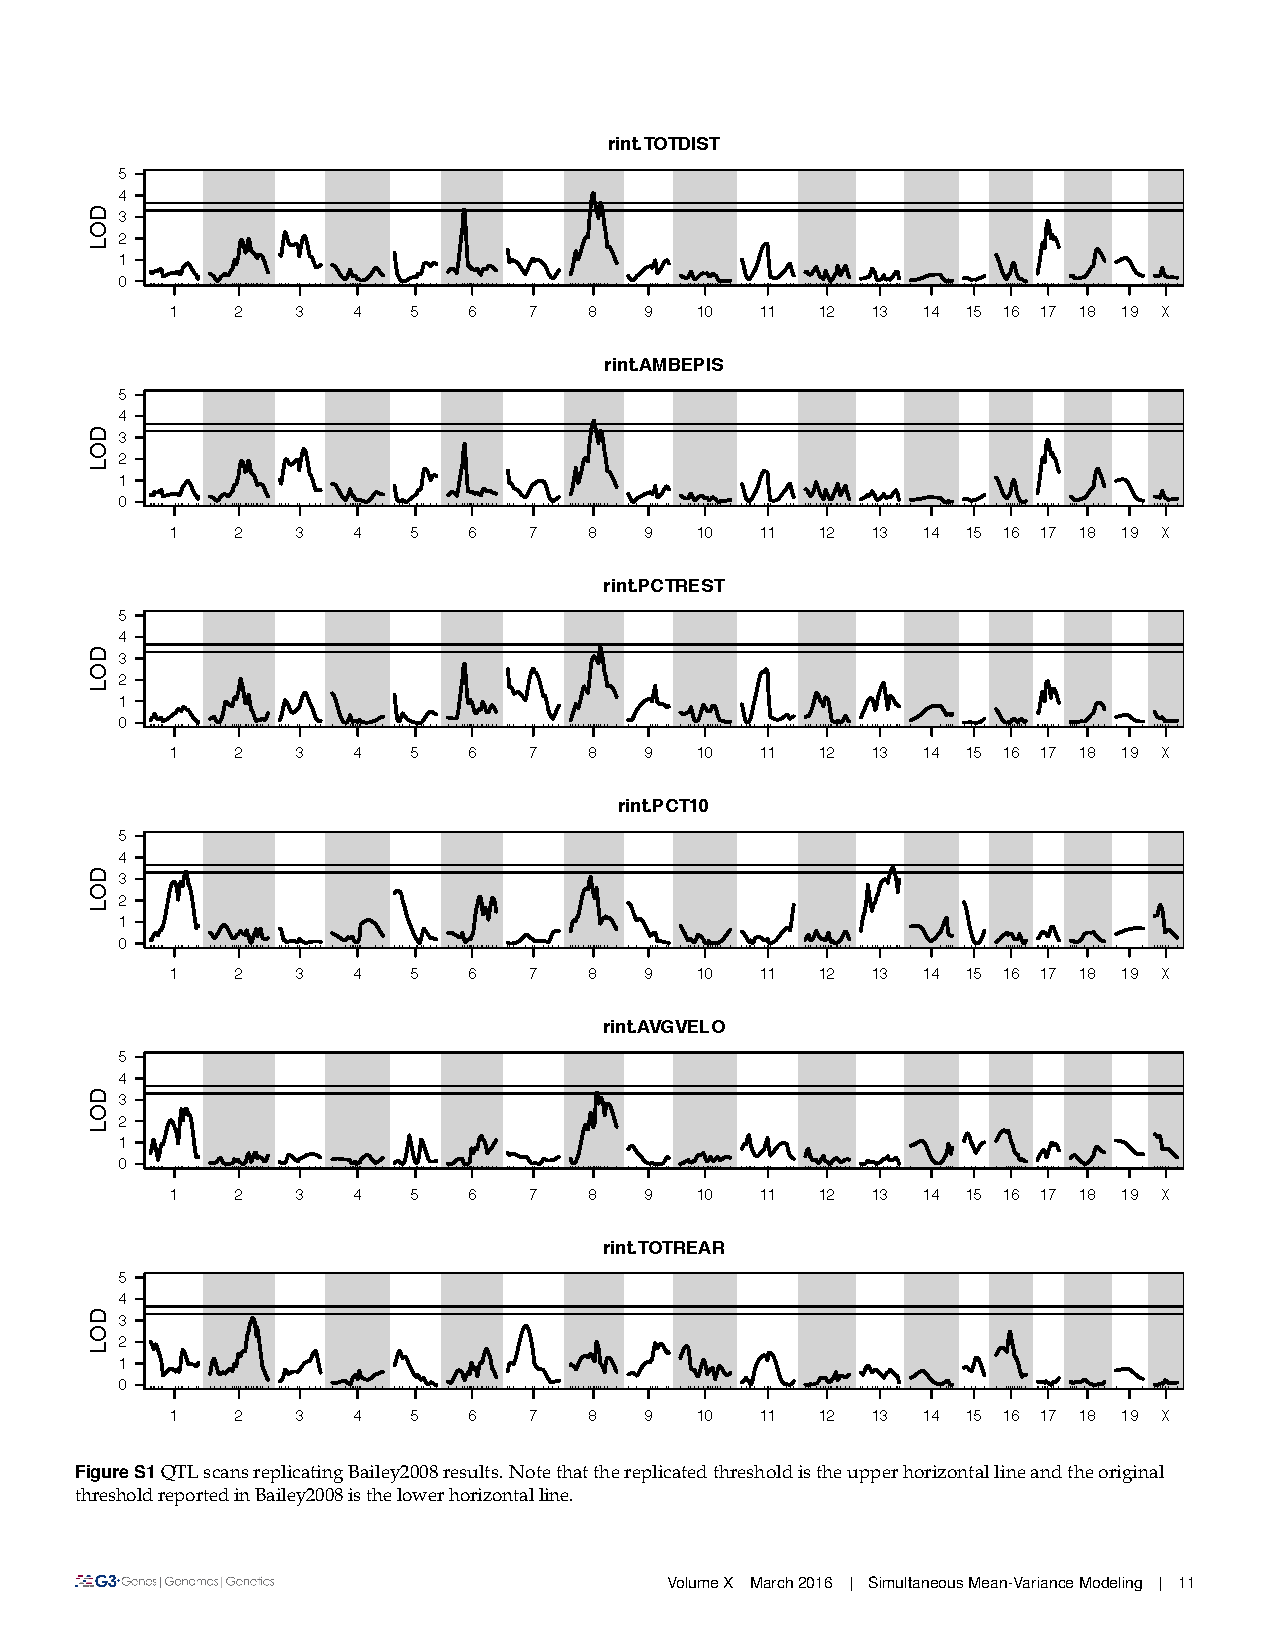
\includegraphics[width = 0.65\textwidth]{scanones}
%   \end{center}
% \end{frame}
% 
% 
% 
% \begin{frame}\frametitle{Results (2)}
%   \begin{itemize}
%     \item[2)] Apply ideas from Ronnegard2011 to map vQTL in this data set\\
%     \begin{itemize}
%       \item[-] Identified one vQTL
%       \item[-] Not surprisingly, decreased evidence for some mQTL
%       \item[-] Surprisingly, increased evidence for some mQTL -- not-significant $\neq$ not-real
%       \item[-] Identified one mvQTL
%       \item[-] Issues on recreating the null distribution via randomization
%       \item[-] Multiple testing correction
%     \end{itemize}
%   \end{itemize}
% \end{frame}
% 
% \begin{frame}\frametitle{Results (2)}
%   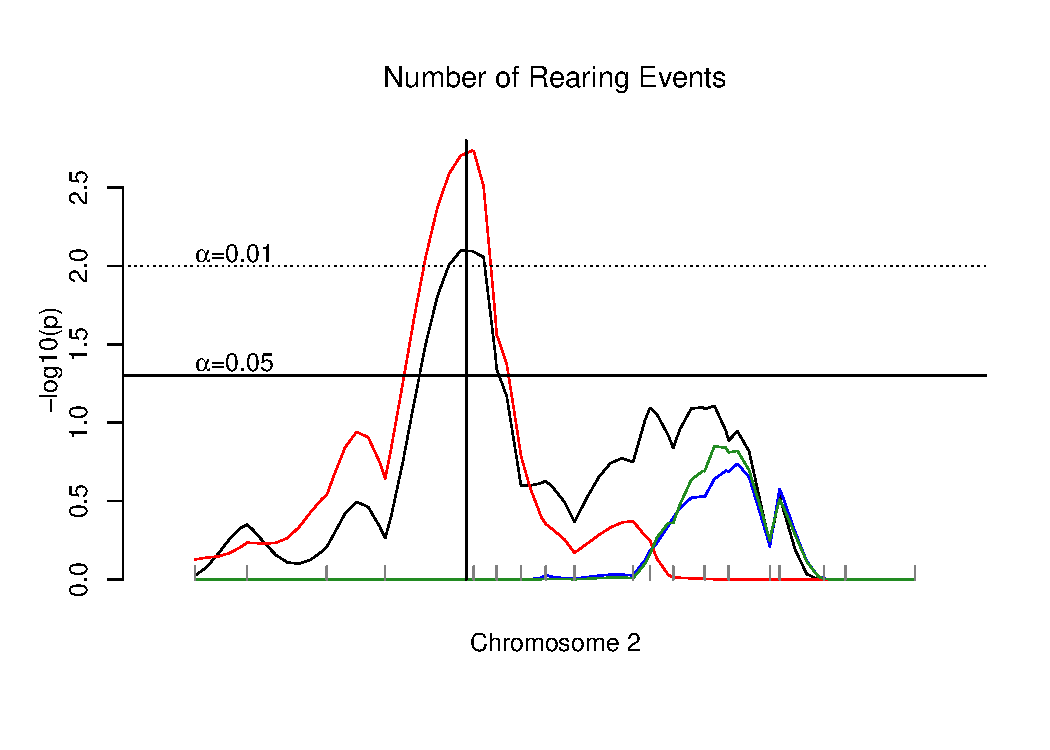
\includegraphics[width = 0.5\textwidth]{rearing_vqtl}
%   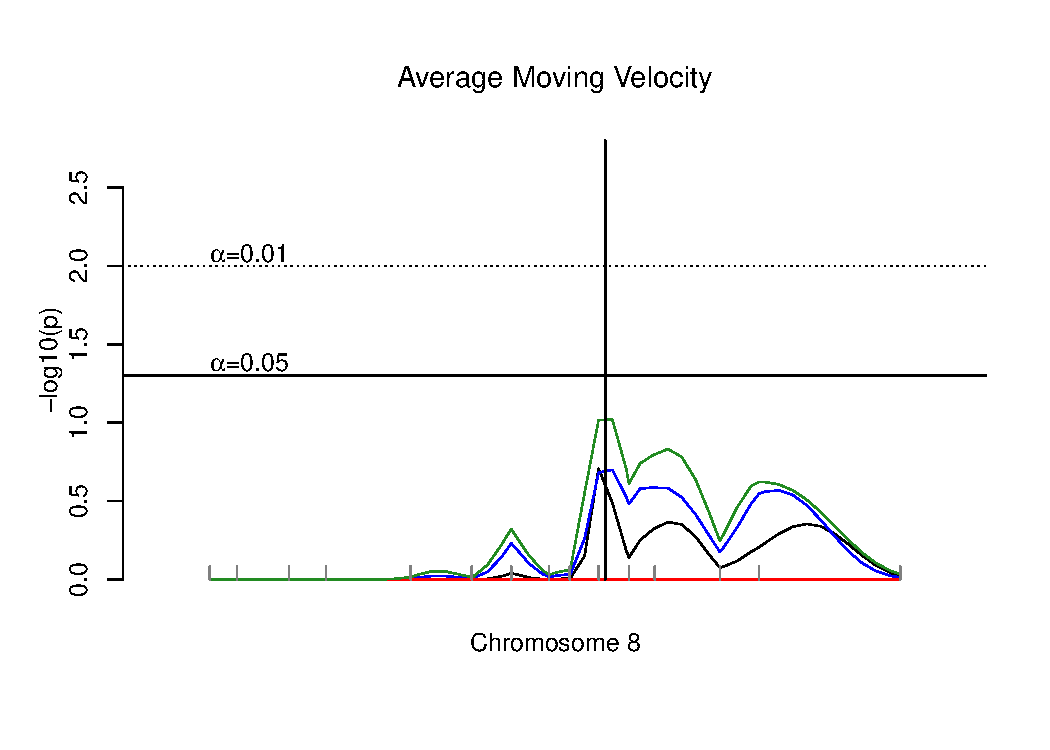
\includegraphics[width = 0.5\textwidth]{vel_decr_mqtl}\\
%   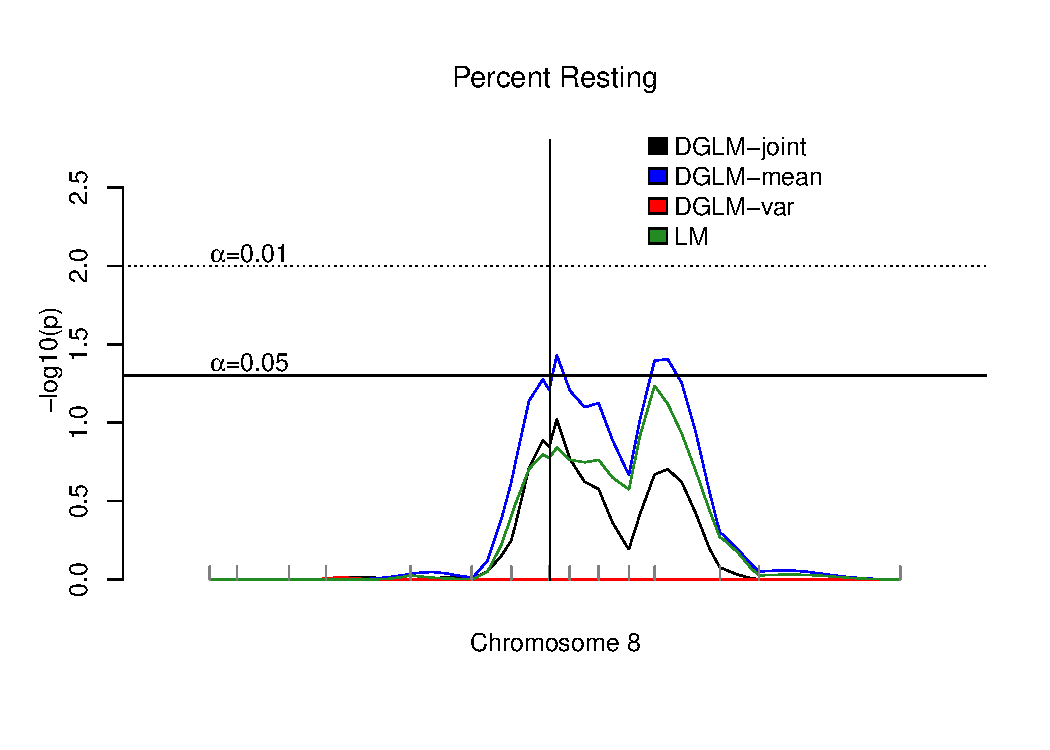
\includegraphics[width = 0.5\textwidth]{resting_incr_mqtl}
%   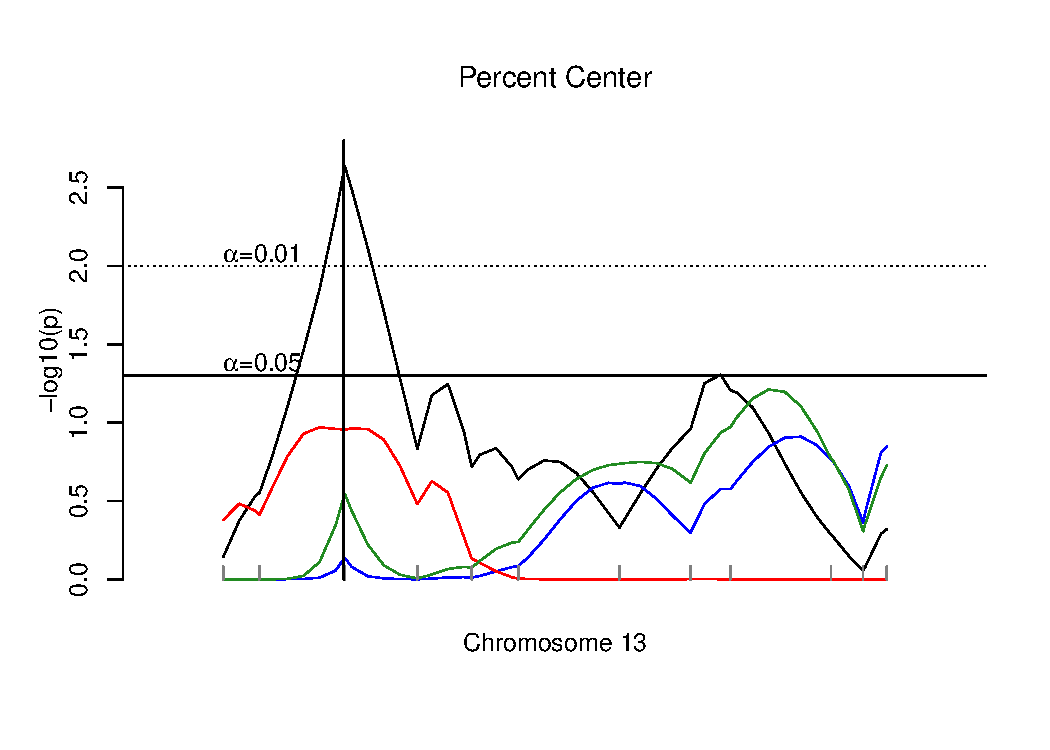
\includegraphics[width = 0.5\textwidth]{center_mvqtl}
% \end{frame}
% 
% 
% 
% 
% 
% 
% 
% 
% \begin{frame}\frametitle{Traditional Modeling Approach -- LM}
%   \vspace{-1cm}
%   \begin{columns}
%     \begin{column}{.2\textwidth}
%       \begin{center}
%         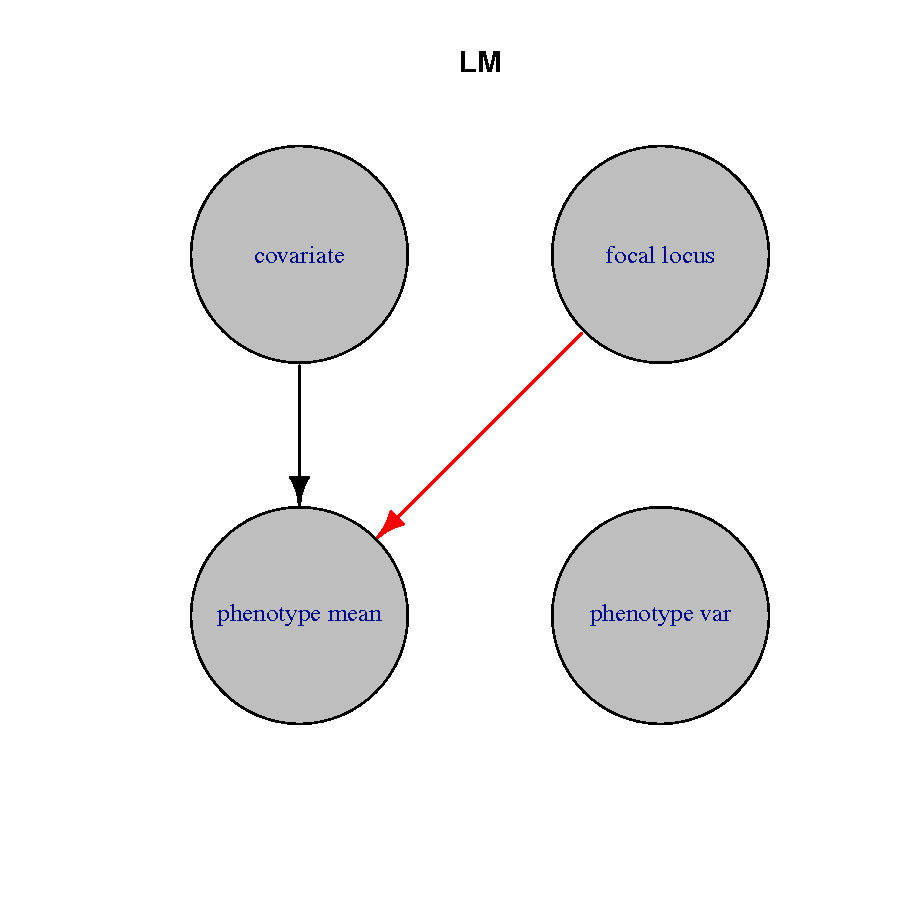
\includegraphics[width = 2.2cm]{lm}
%       \end{center}
%     \end{column}
%     \begin{column}{.5\textwidth}
%       \begin{align*}
%         y_i &\sim \N(m_i, \sigma^2)
%       \end{align*}
%     \end{column}
%   \end{columns}
%   \begin{align*}
%     \onslide<1->{\mathcal{M}_0   && \text{Null model:} &&  m_i &= \bm{x}_i\T\bm{\beta}
\\}
%     \onslide<2->{\mathcal{M}_1   && \text{Alternative model:} &&  m_i &= \bm{x}_i\T\bm{\beta} + \bm{q}_i\T\bm{\alpha}
\\}
%     \onslide<3->{\mathcal{M}_{1*}   && {\renewcommand{\arraystretch}{1}\begin{tabular}{@{}r@{}} Randomized \\ alternative model \end{tabular}} &&  m_i &= \bm{x}_i\T\bm{\beta} + \bm{q}_{\pi(i)}\T\bm{\alpha}
}
%   \end{align*}
%   \begin{itemize}
%     \item simplest possible model for phenotype variance -- all individuals identical
%   \end{itemize}
% \end{frame}
% 
% 
% 
% \begin{frame}\frametitle{Experimental Modeling Approach -- DGLM joint}
%   \vspace{-1cm}
%   \begin{columns}
%     \begin{column}{.2\textwidth}
%       \begin{center}
%         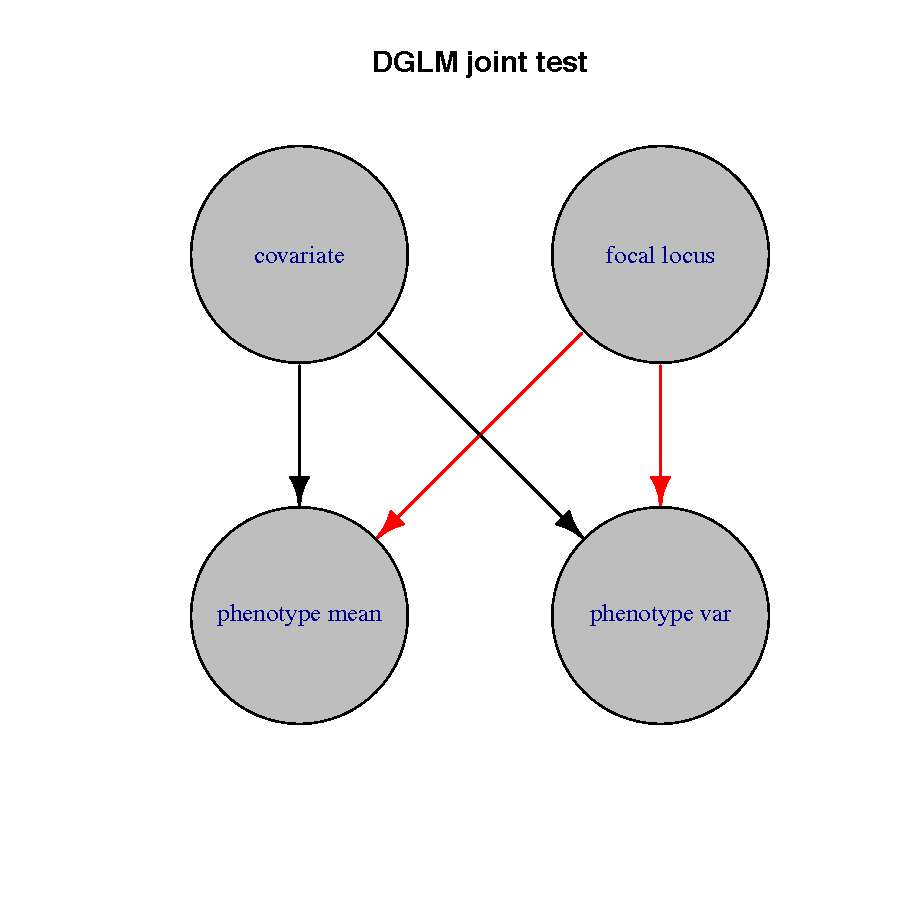
\includegraphics[width = 2.2cm]{dglm_j}
%       \end{center}
%     \end{column}
%     \begin{column}{.5\textwidth}
%     \begin{align*}
%         y_i &\sim \N(m_i, \exp(v_i))
%       \end{align*}
%     \end{column}
%   \end{columns}
%   \begin{flalign*}
%     \onslide<2->{\mathcal{M}_0       && \text{Null model}    &&& \begin{cases} m_i &= \bm{x}_i\T\bm{\beta}\\
v_i &= \bm{z}_i\T\bm{\gamma}
  \end{cases}\\}
%     \onslide<3->{\mathcal{M}_{MV}    && \text{Alternative model}   &&& \begin{cases} m_i &= \bm{x}_i\T\bm{\beta} + \bm{q}_i\T\bm{\alpha}\\
v_i &= \bm{z}_i\T\bm{\gamma} + \bm{q}_i\T\bm{\theta}
 \end{cases}\\}
%     \onslide<4->{\mathcal{M}_{M^*V^*} && {\renewcommand{\arraystretch}{1}\begin{tabular}{@{}r@{}} Randomized \\ alternative model \end{tabular}} &&& \begin{cases} m_i &= \bm{x}_i\T\bm{\beta} + \bm{q}_{\pi(i)}\T\bm{\alpha}\\
v_i &= \bm{z}_i\T\bm{\gamma} + \bm{q}_{\pi(i)}\T\bm{\theta}
  \end{cases}}
%   \end{flalign*}
% \end{frame}
% 
% 
% \begin{frame}\frametitle{Experimental Modeling Approach -- DGLM mean}
%   \vspace{-1cm}
%   \begin{columns}
%     \begin{column}{.2\textwidth}
%       \begin{center}
%         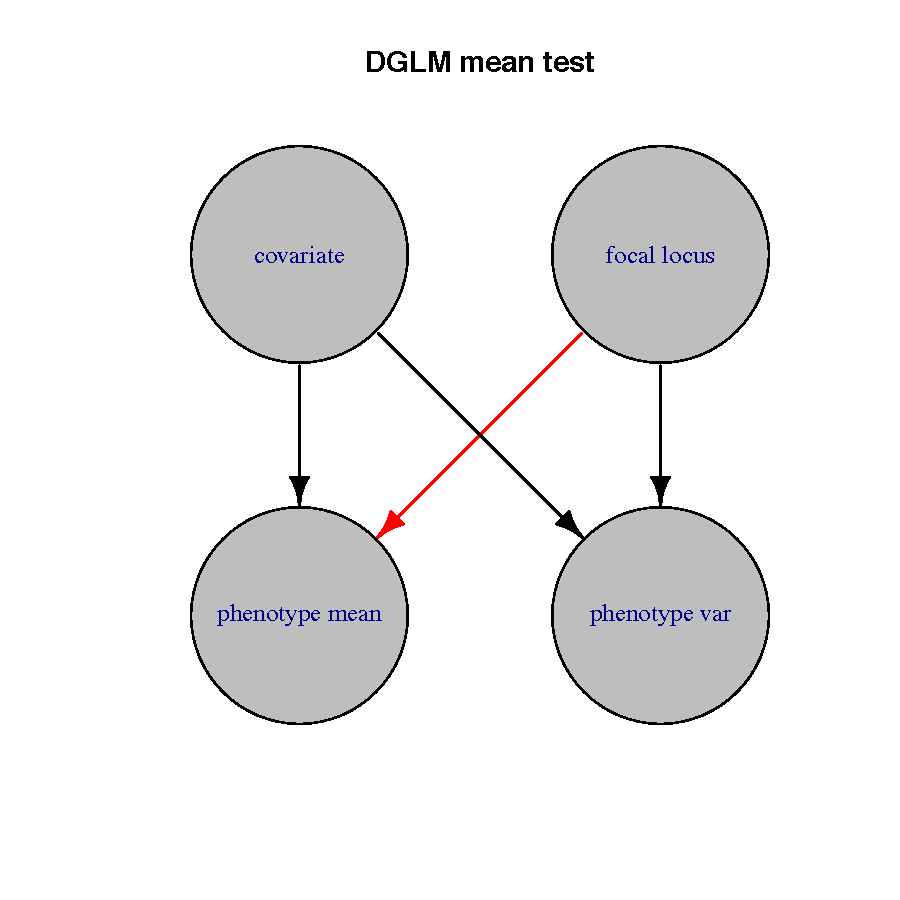
\includegraphics[width = 2.2cm]{dglm_m}
%       \end{center}
%     \end{column}
%     \begin{column}{.5\textwidth}
%     \begin{align*}
%         y_i &\sim \N(m_i, \exp(v_i))
%       \end{align*}
%     \end{column}
%   \end{columns}
%   \begin{flalign*}
%     \onslide<2->{\mathcal{M}_V       && \text{Null model}     &&& \begin{cases} m_i & = \bm{x}_i\T\bm{\beta}\\
v_i & = \bm{z}_i\T\bm{\gamma} + \bm{q}_i\T\bm{\theta}
  \end{cases}\\}
%     \onslide<3->{\mathcal{M}_{MV}    && \text{Alternative model}   &&& \begin{cases} m_i &= \bm{x}_i\T\bm{\beta} + \bm{q}_i\T\bm{\alpha}\\
v_i &= \bm{z}_i\T\bm{\gamma} + \bm{q}_i\T\bm{\theta}
 \end{cases}\\}
%     \onslide<4->{\mathcal{M}_{M^*V}  && {\renewcommand{\arraystretch}{1}\begin{tabular}{@{}r@{}} Randomized \\ alternative model \end{tabular}} &&& \begin{cases} m_i &= \bm{x}_i\T\bm{\beta} + \bm{q}_{\pi(i)}\T\bm{\alpha}\\
v_i &= \bm{z}_i\T\bm{\gamma} + \bm{q}_i\T\bm{\theta}
  \end{cases}}
%   \end{flalign*}
% \end{frame}
% 
% 
% \begin{frame}\frametitle{Experimental Modeling Approach -- DGLM var}
%   \vspace{-1cm}
%   \begin{columns}
%     \begin{column}{.2\textwidth}
%       \begin{center}
%         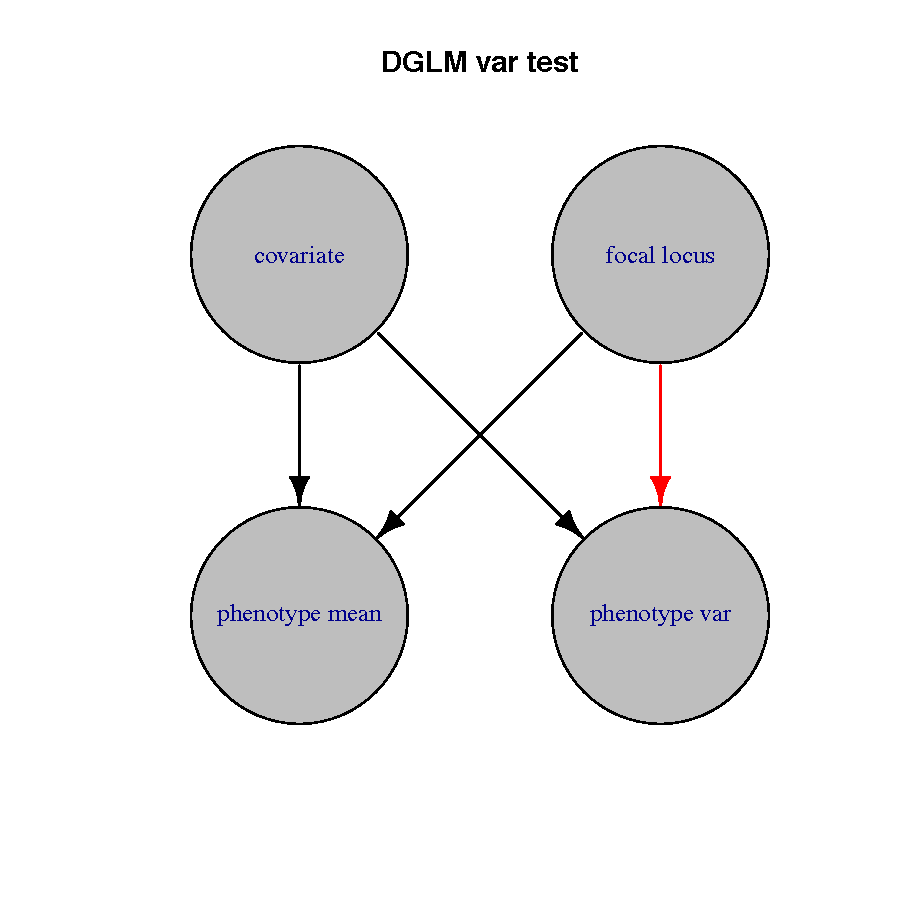
\includegraphics[width = 2.2cm]{dglm_v}
%       \end{center}
%     \end{column}
%     \begin{column}{.5\textwidth}
%     \begin{align*}
%         y_i &\sim \N(m_i, \exp(v_i))
%       \end{align*}
%     \end{column}
%   \end{columns}
%   \begin{flalign*}
%     \onslide<2->{\mathcal{M}_M       && \text{Null model}      &&& \begin{cases} m_i &= \bm{x}_i\T\bm{\beta} + \bm{q}_i\T\bm{\alpha}\\
v_i &= \bm{z}_i\T\bm{\gamma}
  \end{cases}\\}
%     \onslide<3->{\mathcal{M}_{MV}    && \text{Alternative model}   &&& \begin{cases} m_i &= \bm{x}_i\T\bm{\beta} + \bm{q}_i\T\bm{\alpha}\\
v_i &= \bm{z}_i\T\bm{\gamma} + \bm{q}_i\T\bm{\theta}
 \end{cases}\\}
%     \onslide<4->{\mathcal{M}_{MV^*}&& {\renewcommand{\arraystretch}{1}\begin{tabular}{@{}r@{}} Randomized \\ alternative model \end{tabular}} &&& \begin{cases} m_i &= \bm{x}_i\T\bm{\beta} + \bm{q}_i\T\bm{\alpha}\\
v_i &= \bm{z}_i\T\bm{\gamma} + \bm{q}_{\pi(i)}\T\bm{\theta}
  \end{cases}}
%   \end{flalign*}
% \end{frame}
% 
% 
% 
% % \begin{frame}\frametitle{Performance of Randomization Scheme}
% %   \begin{center}
% %     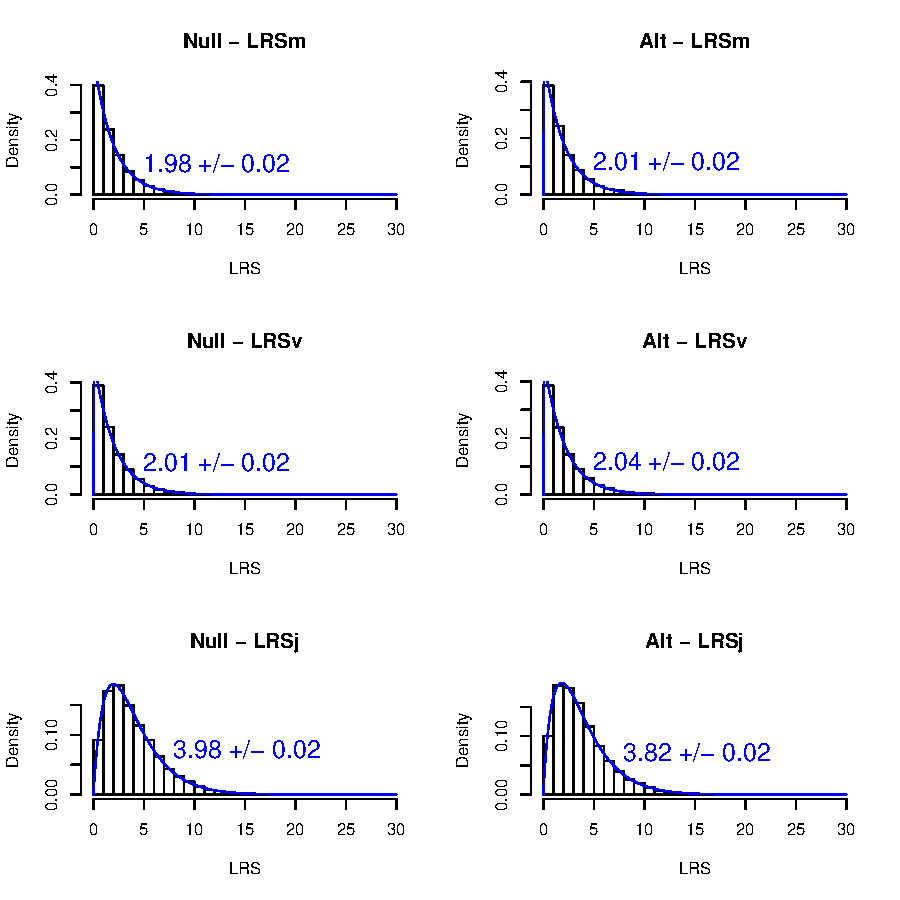
\includegraphics[width = 3in]{LRS_hists}
% %   \end{center}
% % \end{frame}
% 
% \begin{frame}\frametitle{Performance of Randomization Scheme on `non-ugly' Data}
%   \begin{center}
%     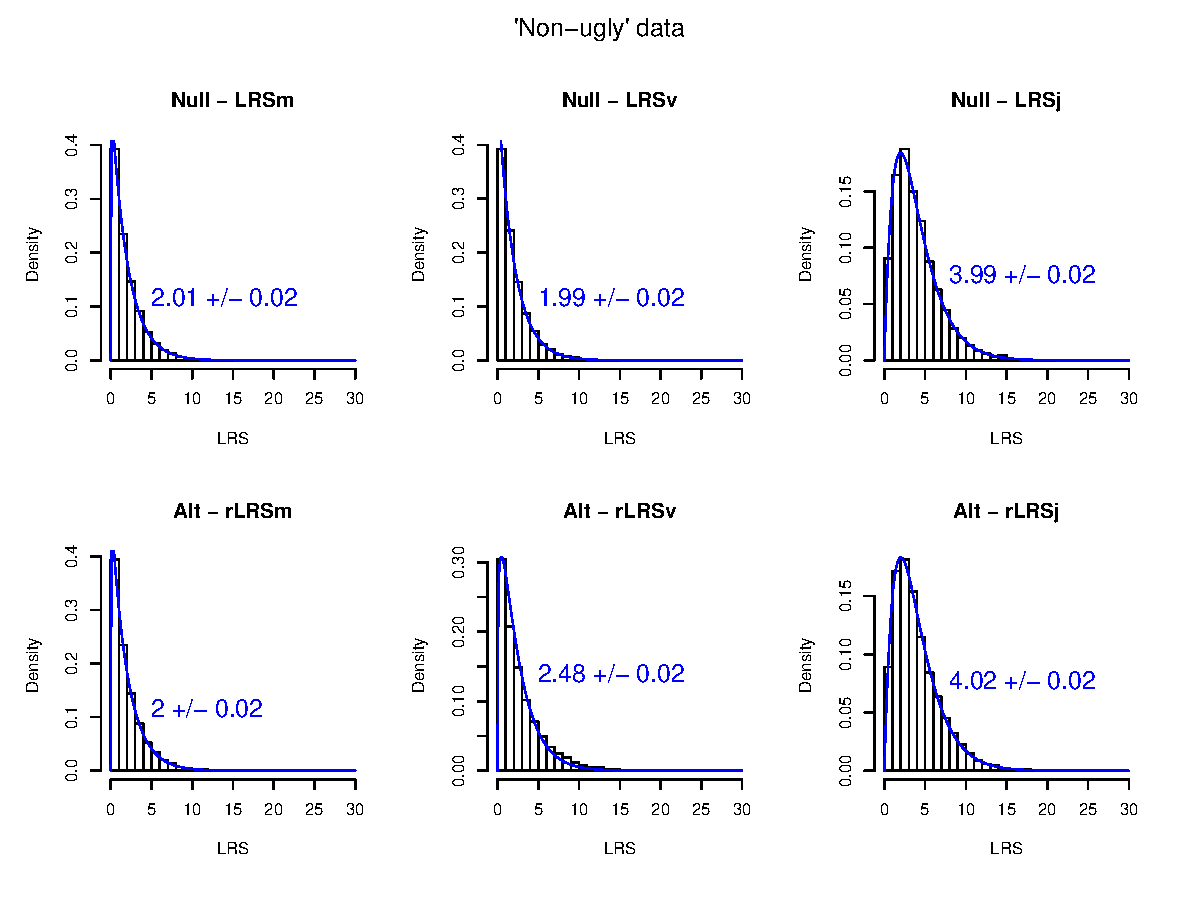
\includegraphics[width = 4in]{non-ugly-data}
%   \end{center}
% \end{frame}
% 
% \begin{frame}\frametitle{Performance of Randomization Scheme on `non-ugly' Data}
%   \begin{center}
%     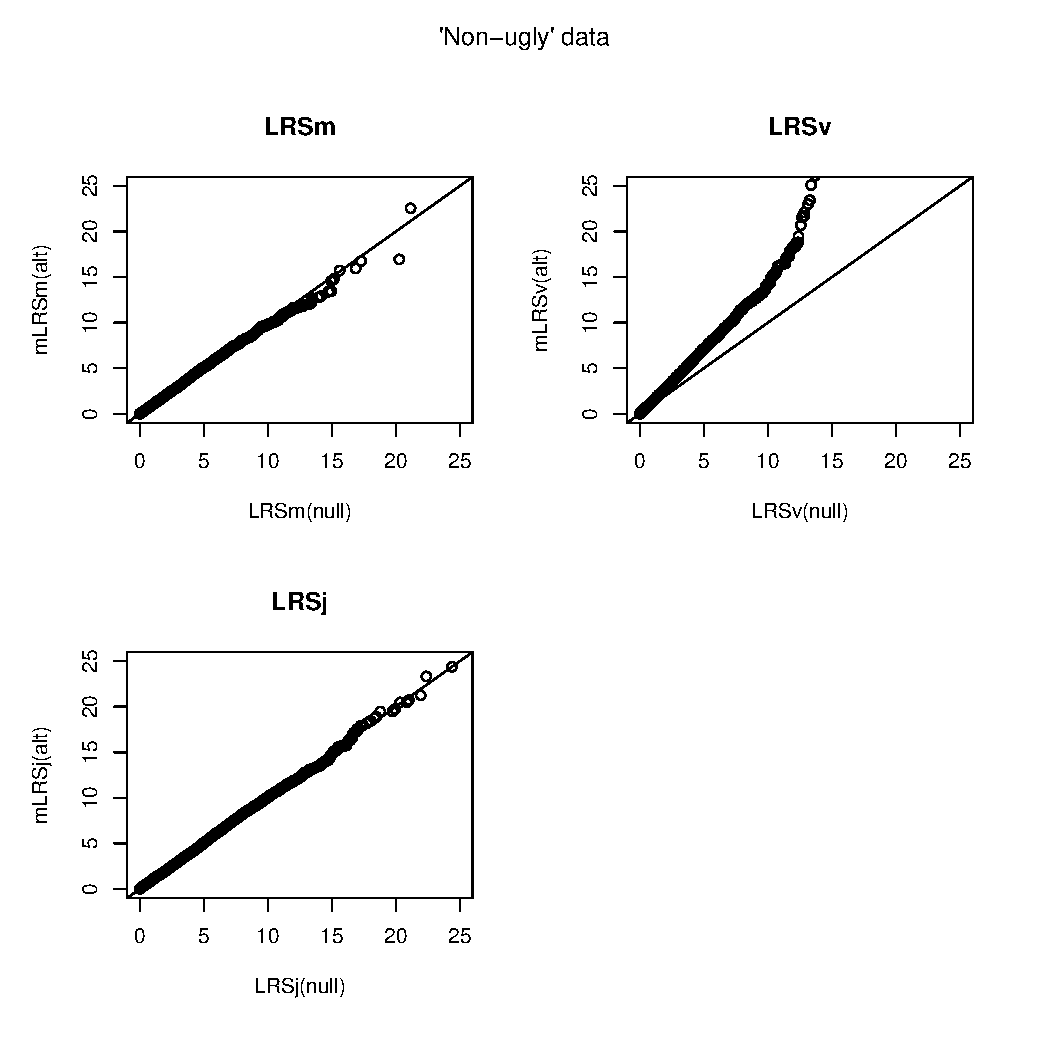
\includegraphics[width = 3in]{non-ugly-qq}
%   \end{center}
% \end{frame}
% 
% \begin{frame}\frametitle{Performance of Randomization Scheme on `ugly' Data}
%   \begin{center}
%     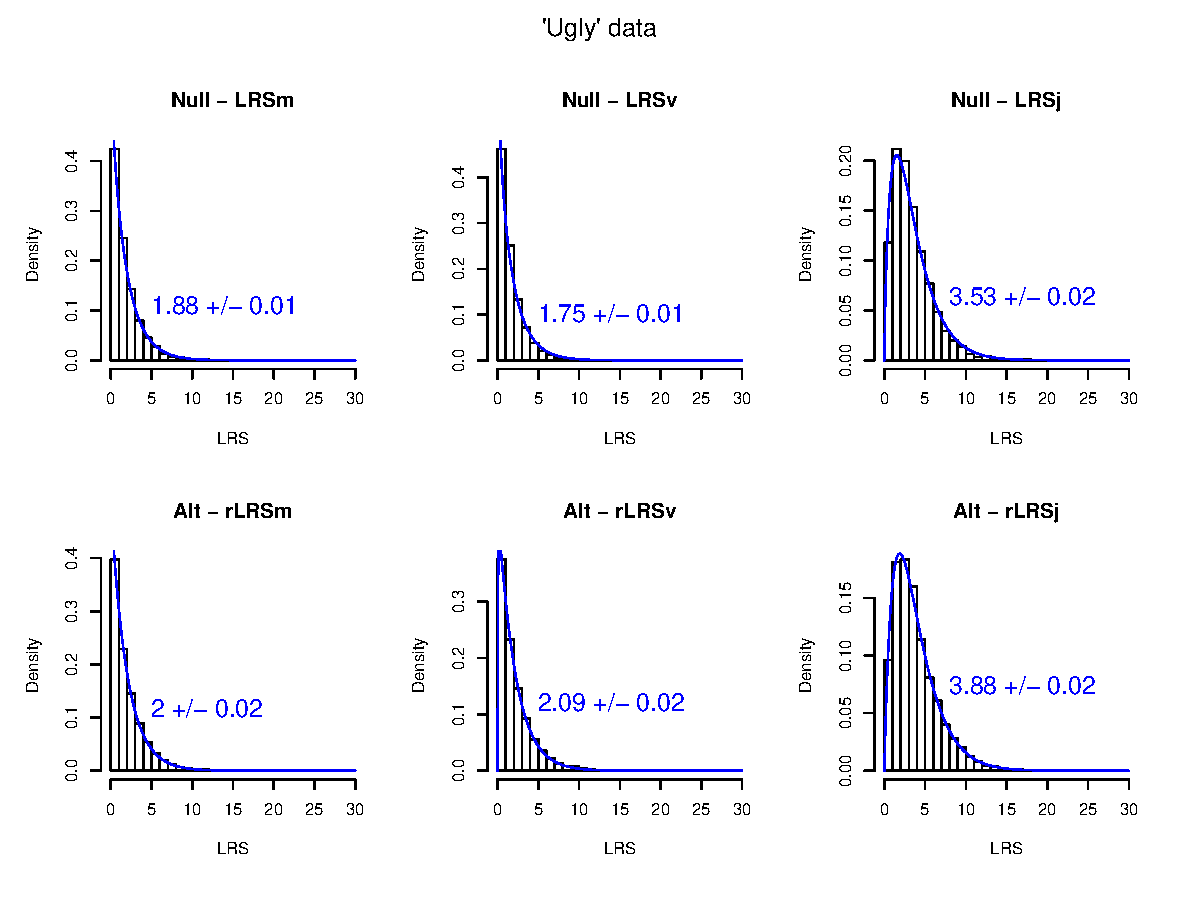
\includegraphics[width = 4in]{ugly-data}
%   \end{center}
% \end{frame}
% 
% \begin{frame}\frametitle{Performance of Randomization Scheme on `ugly' Data}
%   \begin{center}
%     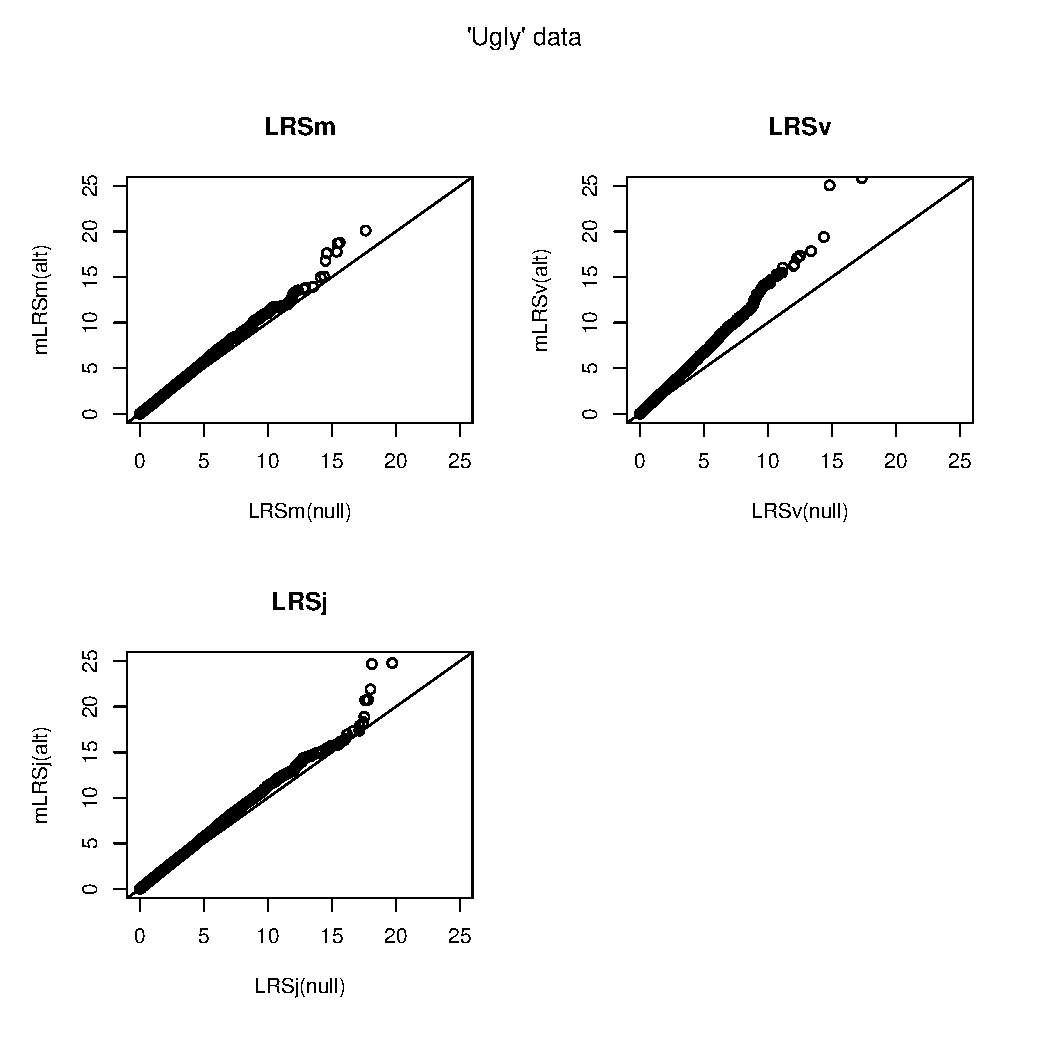
\includegraphics[width = 3in]{ugly-qq}
%   \end{center}
% \end{frame}
% 
% 
% \section{Aim 2: Phenotype Variance in Inbred Strains}
% 
% \begin{frame}\frametitle{Goals}
%   \begin{itemize}
%     \item Extend linear mixed model used for genetic mapping in complex populations for tailored use in inbred populations:
%     \begin{itemize}
%       \item Account for differences in environmental variance between strains
%       \item Account for differences in the number of individuals measured between strains
%       \item Make it faster $(N^3 \rightarrow n^3)$
%     \end{itemize}
%   \end{itemize}
% 
% \end{frame}
% 
% \begin{frame}\frametitle{Progress}
%   \begin{itemize}
%     \item Valdar lab (Will, with help from Greg and I) has preliminarily developed the software to accomplish this
%     \item Next is to verify the correctness of the software, apply it, and start interpreting its behavior
%     \item I have limited my engagement in this project while trying to finish Aim 1
%   \end{itemize}
% \end{frame}
% 
% 
% \section{Additional Projects}
% 
% \begin{frame}\frametitle{Additional Projects}
%   \begin{itemize}
%     \item Lange CVD GxE
%     \item Michelle Engel and Claire Doershuck
%     \item BD2K -- teaching high-dimensional data analysis \cmark
%     \item MD-PhD requirements
%   \end{itemize}
% \end{frame}
\end{document}
